\documentclass[a4paper]{beamer}
\usepackage[utf8]{inputenc}
\usepackage{listings}
\usepackage{ textcomp }
\usepackage{graphicx}
\usepackage[absolute,overlay]{textpos}
\graphicspath{{img/}}
\usetheme{Madrid}
\usecolortheme{crane}
\useoutertheme{shadow}
\usefonttheme{structurebold}
\setbeamertemplate{navigation symbols}{}%remove navigation symbols

\definecolor{applegreen}{rgb}{0.55, 0.71, 0.0}
\definecolor{applegreendark}{rgb}{0.35, 0.51, 0.0}
\definecolor{applegreenpale}{rgb}{0.75, 0.91, 0.2}


\makeatother
\setbeamertemplate{footline}
{
  \leavevmode%
  \hbox{%
  \begin{beamercolorbox}[wd=.4\paperwidth,ht=2.25ex,dp=1ex,center]{author in head/foot}%
    \usebeamerfont{author in head/foot}\insertshortauthor
  \end{beamercolorbox}%
  \begin{beamercolorbox}[wd=.6\paperwidth,ht=2.25ex,dp=1ex,center]{title in head/foot}%
    \usebeamerfont{title in head/foot}\insertshorttitle\hspace*{3em}
    \insertframenumber{} / \inserttotalframenumber\hspace*{1ex}
  \end{beamercolorbox}}%
  \vskip0pt%
}
\makeatletter

\title[Migrating to a NFV-based HomeGateway: the SvNF approach] % (optional, only for long titles)
{Migrating to a NFV-based Home Gateway}
\subtitle{Introducing a Surrogate vNF approach}
\author[\underline{Herbaut}, Negru, Xilouris, Chen] % (optional, for multiple authors)
{\underline{N.~Herbaut\inst{1}} \and D.~Négru\inst{1} \and G.~Xilouris\inst{2} \and Y.Chen\inst{3} }
\institute % (optional)
{
  \inst{1}%
  Univ. Bordeaux, LaBRI\\
  Talence, France
  \and
  \inst{2}%
  NCSR Demokritos\\
  Athens, Greece
  \and
  \inst{3}%
  Orange Labs\\
  Issy-les-moulineaux, France 
}
\date[NOF2015] % (optional)
{The 6th International Conference On Network of the Future}
\subject{Computer Science.}
\titlegraphic{
\includegraphics[height=1cm]{ub.jpg}~%
   
\includegraphics[height=1cm]{Logo_LaBRI_complet.jpg}~%
   
\includegraphics[height=1cm]{viotech.jpg}~%
   
\includegraphics[height=1cm]{top_logo1.jpg}
   
   
}

\begin{document}
\frame{\titlepage}


\begin{frame}{Objectives of the paper}
											
	\begin{itemize}
																					
		\item Proposing a technical solution to ease the migration to future Home Gateway technologies.
		      \pause
		\item Study the feasibility through a concrete use case.
	\end{itemize}
											
											
\end{frame}

%%%%%%%%%%%%%%%%%%%%%%%%%%%%%%%%%%%%%%%%%%%%%%%%%%%%%%%%%%%%%%%%%%
%%%%%%%%%%%%%%%%%%%%%%%%%%%%%%%%%%%%%%%%%%%%%%%%%%%%%%%%%%%%%%%%%%
%%%%%%%%%%%%%%%%%%%%%%%%%%%%%%%%%%%%%%%%%%%%%%%%%%%%%%%%%%%%%%%%%%
%%%%%%%%%%%%%%%%%%%%%%%%%%%%%%%%%%%%%%%%%%%%%%%%%%%%%%%%%%%%%%%%%%

\begin{frame}{Outline}
																	
																	
																
	\begin{columns}[c] % the "c" option specifies center vertical alignment
		\column{.03\textwidth} % column designated by a command
		\begin{block}{}
			\rotatebox{90}{~~~~~Context~~~~~~}
		\end{block}
		\column{.25\textwidth} % column designated by a command
		\begin{block}{1. Home Boxes Today}
			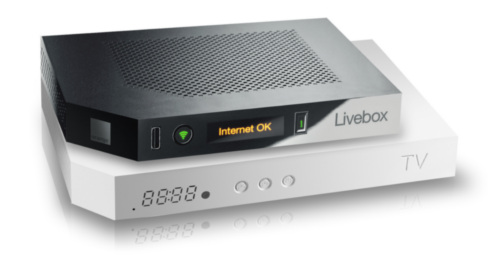
\includegraphics[width= \textwidth]{homebox.jpg}
		\end{block}
		\column{.25\textwidth}
		\begin{block}{2. Virtual Home Gateway }
			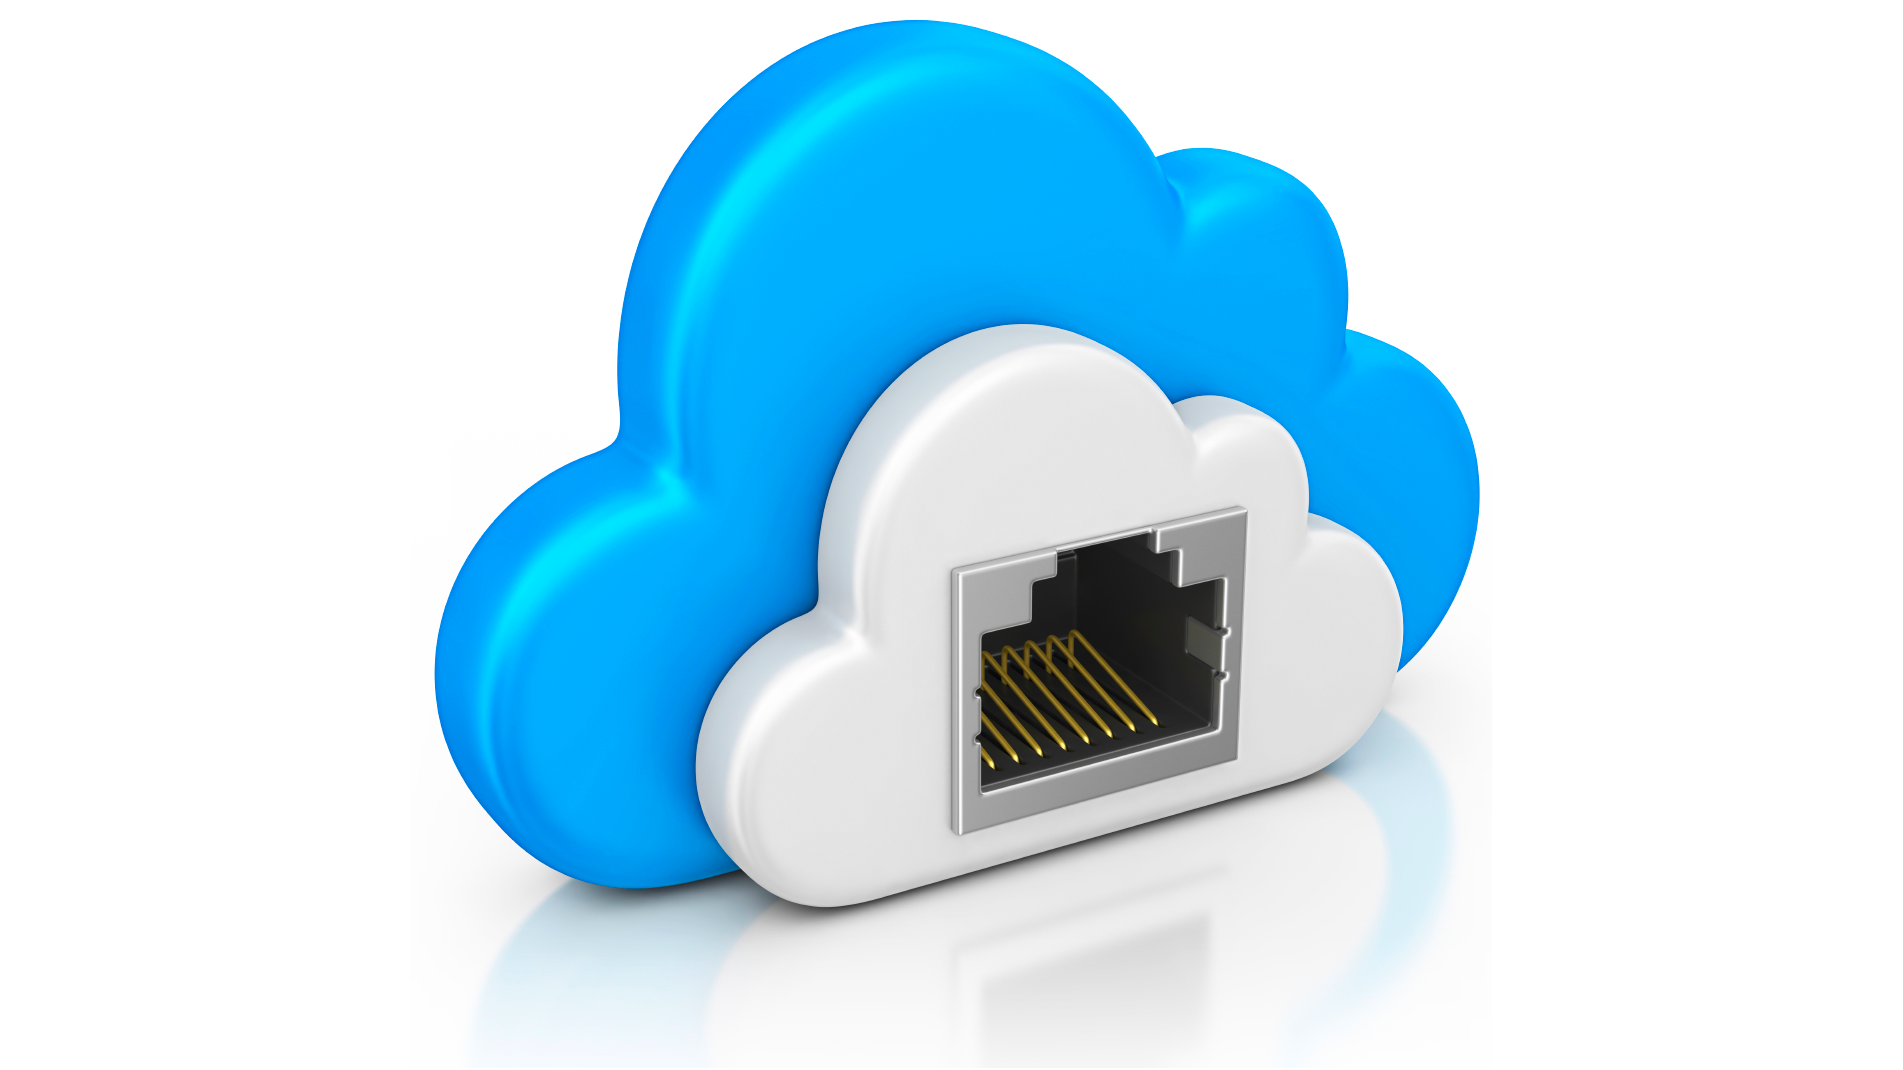
\includegraphics[width= \textwidth]{vhg.png}
		\end{block}
																																          
		\column{.25\textwidth}
		\begin{block}{3. NFV for Future Networks}
			
\includegraphics[width= \textwidth]{etsinfv.png}
		\end{block}
																																          
																																      
	\end{columns}
															
	\setbeamercolor{block title}{bg=applegreen}
															
																    
	\begin{columns}[c] % the "c" option specifies center vertical alignment
		\column{.03\textwidth} % column designated by a command
		\begin{block}{}
			\rotatebox{90}{~~~~Proposal~~~~~}
		\end{block}
																														
		\column{.25\textwidth} % column designated by a command
		\begin{block}{4. Easing the Migration}
			
\includegraphics[width= \textwidth]{loco.png}
		\end{block}
																																 
		\column{.25\textwidth} % column designated by a command
		\begin{block}{5. Experiments, Results}
			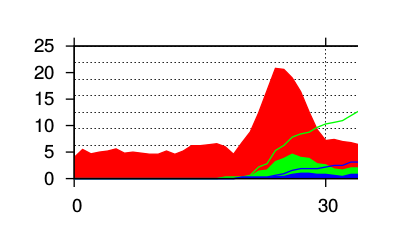
\includegraphics[width= \textwidth]{results.png}
		\end{block}
																																          
		\column{.25\textwidth} % column designated by a command
		\begin{block}{6. Discussion \& Conclusion}
			
\includegraphics[width= \textwidth]{conclusion.jpg}
		\end{block}
																																 
	\end{columns}
																    
														
																    
																    
\end{frame}


%%%%%%%%%%%%%%%%%%%%%%%%%%%%%%%%%%%%%%%%%%%%%%%%%%%%%%%%%%%%%%%%%%
%%%%%%%%%%%%%%%%%%%%%%%%%%%%%%%%%%%%%%%%%%%%%%%%%%%%%%%%%%%%%%%%%%
%%%%%%%%%%%%%%%%%%%%%%%%%%%%%%%%%%%%%%%%%%%%%%%%%%%%%%%%%%%%%%%%%%
%%%%%%%%%%%%%%%%%%%%%%%%%%%%%%%%%%%%%%%%%%%%%%%%%%%%%%%%%%%%%%%%%%

\begin{frame}{With Customer Premises Equipment (CPE), Service Providers bring a lot of features to Users}
												
											
	\begin{columns}[T] 
		\begin{column}[T]{0.25 \textwidth} 
			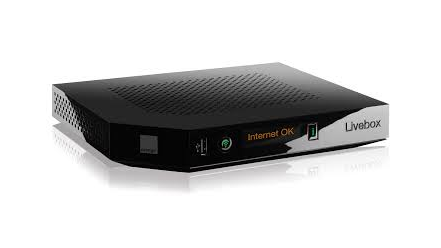
\includegraphics[width=\linewidth]{livebox.png}
		\end{column}
																										
		\begin{column}[T]{0.75 \textwidth} % each column can also be its own environment
																																							
			\textbf{Home Gateway  (HG)}
			\begin{itemize}
				\item Connects the Service Provider Network 
				\item Network services: NAT, DHCP, Wifi...
				\item Users-facing services: Printing Service, VoIP, Parental Control...
				\item New Services: Internet of Things, Home Automation...
			\end{itemize}
			\vspace{1em}
																																							
		\end{column}
																										
	\end{columns}
												
												
													
												
	\begin{columns}[T] 
		\begin{column}[T]{0.25 \textwidth} 
			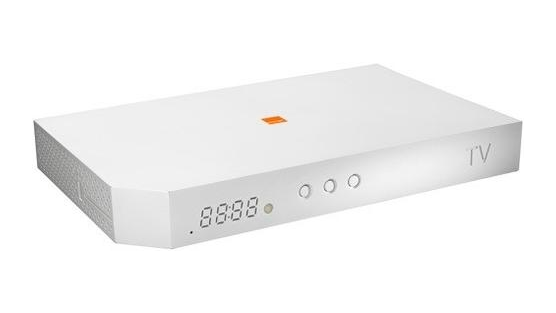
\includegraphics[width=\linewidth]{liveboxdec.png}
		\end{column}
																										
		\begin{column}[T]{0.75 \textwidth} % each column can also be its own environment
																																							
																																								   
			\textbf{ Set-Top-Box (STB)}
			\begin{itemize}
				\item Decode media IP flows to a display device
				\item Live TV, Video On Demand ...
				\item Catch-up TV, Recording ...
				\item Legacy Digital terrestrial television ...
			\end{itemize}
																																								     
																																							
		\end{column}
																										
	\end{columns}
													
													
													
\end{frame}

%%%%%%%%%%%%%%%%%%%%%%%%%%%%%%%%%%%%%%%%%%%%%%%%%%%%%%%%%%%%%%%%%%
%%%%%%%%%%%%%%%%%%%%%%%%%%%%%%%%%%%%%%%%%%%%%%%%%%%%%%%%%%%%%%%%%%
%%%%%%%%%%%%%%%%%%%%%%%%%%%%%%%%%%%%%%%%%%%%%%%%%%%%%%%%%%%%%%%%%%
%%%%%%%%%%%%%%%%%%%%%%%%%%%%%%%%%%%%%%%%%%%%%%%%%%%%%%%%%%%%%%%%%%

\begin{frame}{CPEs cost a lot to produce and to support}
											
	\begin{columns}[T] 
		\begin{column}[T]{0.15 \textwidth} 
			
\includegraphics[width=3em]{bagofmoney.jpg}
		\end{column}
																										
		\begin{column}[T]{0.75 \textwidth} % each column can also be its own environment
																																							
																																								   
			\textbf{ High Capital Expenditure (CAPEX)}
			\begin{itemize}
				\item High design \& Engineering costs
				\item Supply Chain costs, need for spare devices
				\item Hardware upgrades can be necessary to roll-out new services
			\end{itemize}
			\vspace{3em}				     
																																							
		\end{column}
																										
	\end{columns}
											
											
	\begin{columns}[T] 
		\begin{column}[T]{0.15 \textwidth} 
			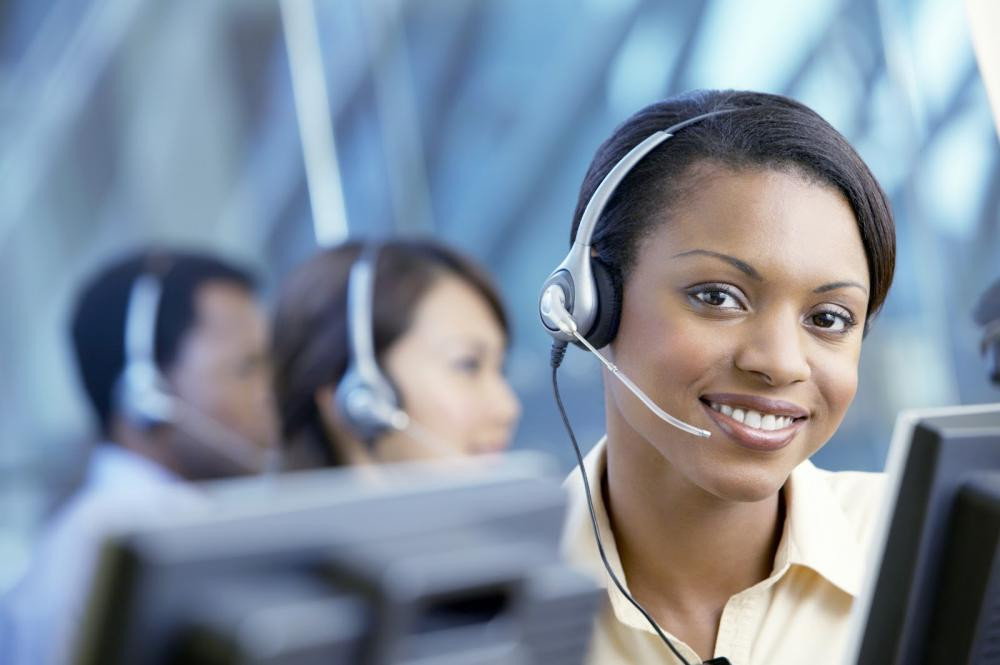
\includegraphics[width=6em]{customer-care.jpg}
		\end{column}
																						
																										
		\begin{column}[T]{0.75 \textwidth} % each column can also be its own environment
																																							
																																								   
			\textbf{ High Operational Expenditure (OPEX)}
			\begin{itemize}
				\item Need to maintain legacy models
				\item Difficult to update software of a very fragmented installed base
				\item Costly customer service 
			\end{itemize}
																																								     
																																							
		\end{column}
																										
	\end{columns}
											
											
\end{frame}


%%%%%%%%%%%%%%%%%%%%%%%%%%%%%%%%%%%%%%%%%%%%%%%%%%%%%%%%%%%%%%%%%%
%%%%%%%%%%%%%%%%%%%%%%%%%%%%%%%%%%%%%%%%%%%%%%%%%%%%%%%%%%%%%%%%%%
%%%%%%%%%%%%%%%%%%%%%%%%%%%%%%%%%%%%%%%%%%%%%%%%%%%%%%%%%%%%%%%%%%
%%%%%%%%%%%%%%%%%%%%%%%%%%%%%%%%%%%%%%%%%%%%%%%%%%%%%%%%%%%%%%%%%%

\begin{frame}{CPEs cost a lot to produce and to support}
											
	\begin{columns}[T] 
		\begin{column}[T]{0.15 \textwidth} 
			
\includegraphics[width=3em]{bagofmoney.jpg}
		\end{column}
																										
		\begin{column}[T]{0.75 \textwidth} % each column can also be its own environment
																																							
																																								   
			\textbf{ High Capital Expenditure (CAPEX)}
			\begin{itemize}
				\item High design \& Engineering costs
				\item Supply Chain costs, need for spare devices
				\item Hardware upgrades can be necessary to roll-out new services
			\end{itemize}
			\vspace{3em}				     
																																							
		\end{column}
																										
	\end{columns}
											
											
	\begin{columns}[T] 
		\begin{column}[T]{0.15 \textwidth} 
			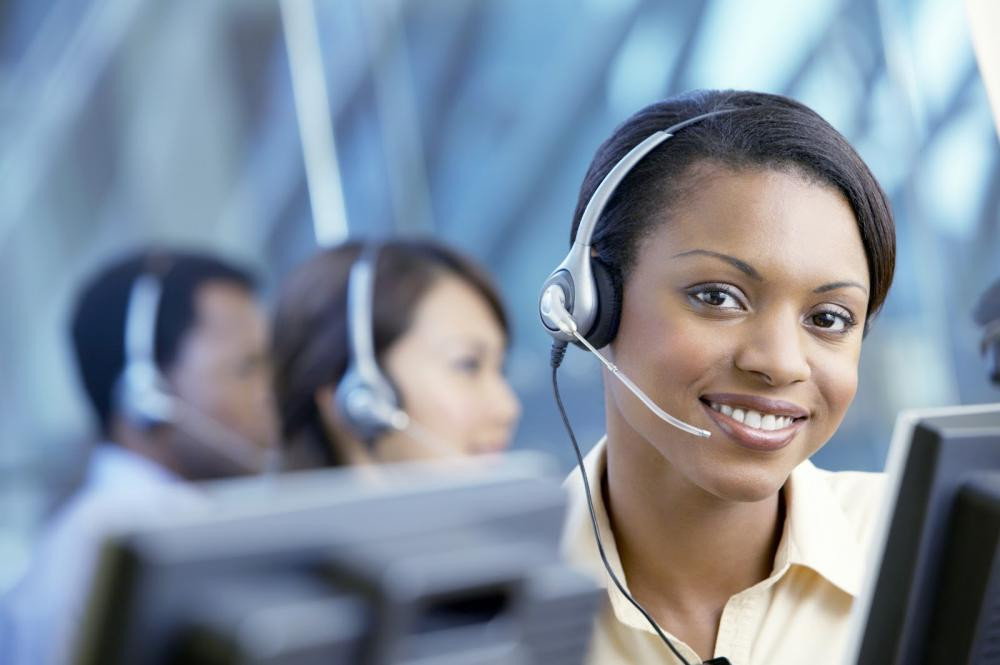
\includegraphics[width=6em]{customer-care.jpg}
		\end{column}
																						
																										
		\begin{column}[T]{0.75 \textwidth} % each column can also be its own environment
																																							
																																								   
			\textbf{ High Operational Expenditure (OPEX)}
			\begin{itemize}
				\item Need to maintain legacy models
				\item Difficult to update software of a very fragmented installed base
				\item Costly customer service 
			\end{itemize}
																																								     
																																							
		\end{column}
																										
	\end{columns}
											
										
	\begin{textblock*}{10cm}(1cm,0.5\textheight)
		\begin{alertblock}{}
			\textbf{  How do we fix it? }
			\begin{itemize}
				\item Can we design better CPE architecture?
				\item Can we simplify the deployment of new services?
				\item Can we leverage existing industry proposals?
			\end{itemize}
		\end{alertblock}
	\end{textblock*}
											
\end{frame}

\begin{frame}{Current CPE architectures are not modular: maintenance and new service deployment are hard.}
										
	\begin{columns}[T]
		\begin{column}{.01\textwidth} % column designated by a command
			\rotatebox{90}{~~~~Monolithic~~~~}
		\end{column}
		\begin{column}[T]{0.15 \textwidth} 
			\vspace{1em}
			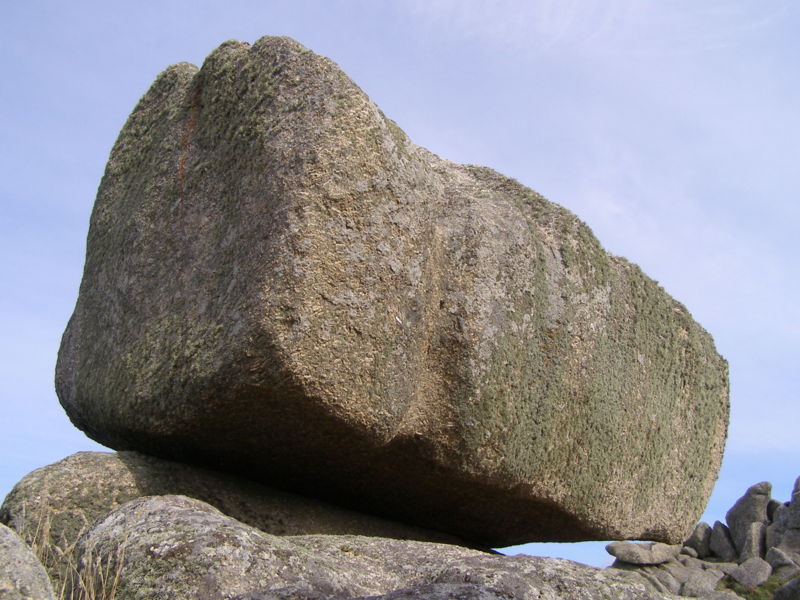
\includegraphics[width=6em]{monolith.jpg}
		\end{column}
																						
																										
		\begin{column}[T]{0.70 \textwidth} 
																																							
																																								   
			\textbf{Today: Firmware-based Home Gateways}
			\begin{itemize}
				\item Embed system software
				\item Complete system update to deploy new feature
				\item Still widely used by vendors
			\end{itemize}
			\vspace{5mm}
																																								     
																																							
		\end{column}
																										
	\end{columns}
										
									
											
\end{frame}


\begin{frame}{Alternative Modular CPE architectures exist, new service can be pushed easily}
							
							
	\begin{columns}[T]
		\begin{column}{.01\textwidth} % column designated by a command
			\rotatebox{90}{~~~~Modular~~~~}
		\end{column}
		\begin{column}[T]{0.15 \textwidth} 
			\vspace{1em}
			
\includegraphics[width=4em]{tux.png}
		\end{column}
																						
																										
		\begin{column}[T]{0.70 \textwidth} 
																																							
																																								   
			\textbf{ GNU/Linux Home Gateways}
			\begin{itemize}
				\item Stable, tested, reusable code-base
				\item Modularity through package management
				\item Limited support for Service Oriented Architecture
			\end{itemize}
			\vspace{3mm}
																																								     
																																							
		\end{column}
																										
	\end{columns}
								
								
	\begin{columns}[T]
		\begin{column}{.01\textwidth} % column designated by a command
			\rotatebox{90}{~~~~Modular~~~~}
		\end{column}
		\begin{column}[T]{0.15 \textwidth} 
			\vspace{2em}
			
\includegraphics[width=6em]{hgi.png}
		\end{column}
																						
																										
		\begin{column}[T]{0.70 \textwidth} 
																																							
																																								   
			\textbf{ HGI Open Platform 2.0}
			\begin{itemize}
				\item Support OSGi Standard for modularity
				\item Support mainly JVM dialects
				\item Service Oriented Architecture
			\end{itemize}
			\vspace{3mm}
																																								     
																																							
		\end{column}
																										
	\end{columns}
						
						
	\begin{columns}[T]
		\begin{column}{.01\textwidth} % column designated by a command
																	
			\rotatebox{90}{~~~~Modular~~~~}
		\end{column}
		\begin{column}[T]{0.15 \textwidth} 
			\vspace{1em}
			
\includegraphics[width=4em]{droid.png}
		\end{column}
																						
																										
		\begin{column}[T]{0.70 \textwidth} 
																																							
																																								   
			\textbf{ Android}
			\begin{itemize}
				\item Thousands of applications
				\item Designed for multi-vendor
				\item Service Oriented Architecture
			\end{itemize}
			\vspace{5mm}
																																								     
																																							
		\end{column}
																										
	\end{columns}
							
								
								
								
										
								
									
\end{frame}



\begin{frame}{Alternative Modular CPE architectures exist, new service can be pushed easily}
							
							
	\begin{columns}[T]
		\begin{column}{.01\textwidth} % column designated by a command
			\rotatebox{90}{~~~~Modular~~~~}
		\end{column}
		\begin{column}[T]{0.15 \textwidth} 
			\vspace{1em}
			
\includegraphics[width=4em]{tux.png}
		\end{column}
																						
																										
		\begin{column}[T]{0.70 \textwidth} 
																																							
																																								   
			\textbf{ GNU/Linux Home Gateways}
			\begin{itemize}
				\item Stable, tested, reusable code-base
				\item Modularity through package management
				\item Limited support for Service Oriented Architecture
			\end{itemize}
			\vspace{3mm}
																																								     
																																							
		\end{column}
																										
	\end{columns}
								
								
	\begin{columns}[T]
		\begin{column}{.01\textwidth} % column designated by a command
			\rotatebox{90}{~~~~Modular~~~~}
		\end{column}
		\begin{column}[T]{0.15 \textwidth} 
			\vspace{2em}
			
\includegraphics[width=6em]{hgi.png}
		\end{column}
																						
																										
		\begin{column}[T]{0.70 \textwidth} 
																																							
																																								   
			\textbf{ HGI Open Platform 2.0}
			\begin{itemize}
				\item Support OSGi Standard for modularity
				\item Support mainly JVM dialects
				\item Service Oriented Architecture
			\end{itemize}
			\vspace{3mm}
																																								     
																																							
		\end{column}
																										
	\end{columns}
						
						
	\begin{columns}[T]
		\begin{column}{.01\textwidth} % column designated by a command
																	
			\rotatebox{90}{~~~~Modular~~~~}
		\end{column}
		\begin{column}[T]{0.15 \textwidth} 
			\vspace{1em}
			
\includegraphics[width=4em]{droid.png}
		\end{column}
																						
																										
		\begin{column}[T]{0.70 \textwidth} 
																																							
																																								   
			\textbf{ Android}
			\begin{itemize}
				\item Thousands of applications
				\item Designed for multi-vendor
				\item Service Oriented Architecture
			\end{itemize}
			\vspace{5mm}
																																								     
																																							
		\end{column}
																										
	\end{columns}
							
								
								
							
	\begin{textblock*}{7cm}(3cm,0.5\textheight)
		\begin{alertblock}{}
			\textbf{  We did not fix the major issues. }
			\begin{itemize}
				\item Deploying new software is easier, but still difficult due to the scale.
				\item CAPEX and OPEX are still high.
				\item We may need to replace the whole CPE due to hardware limitations.
			\end{itemize}
		\end{alertblock}
	\end{textblock*}			
											
									
										
\end{frame}

\begin{frame}{Virtual CPE is an alternative and disruptive scenario}
						
	\begin{columns}[T]
		\begin{column}[T]{0.33 \textwidth} 
			\vspace{2.2cm}
			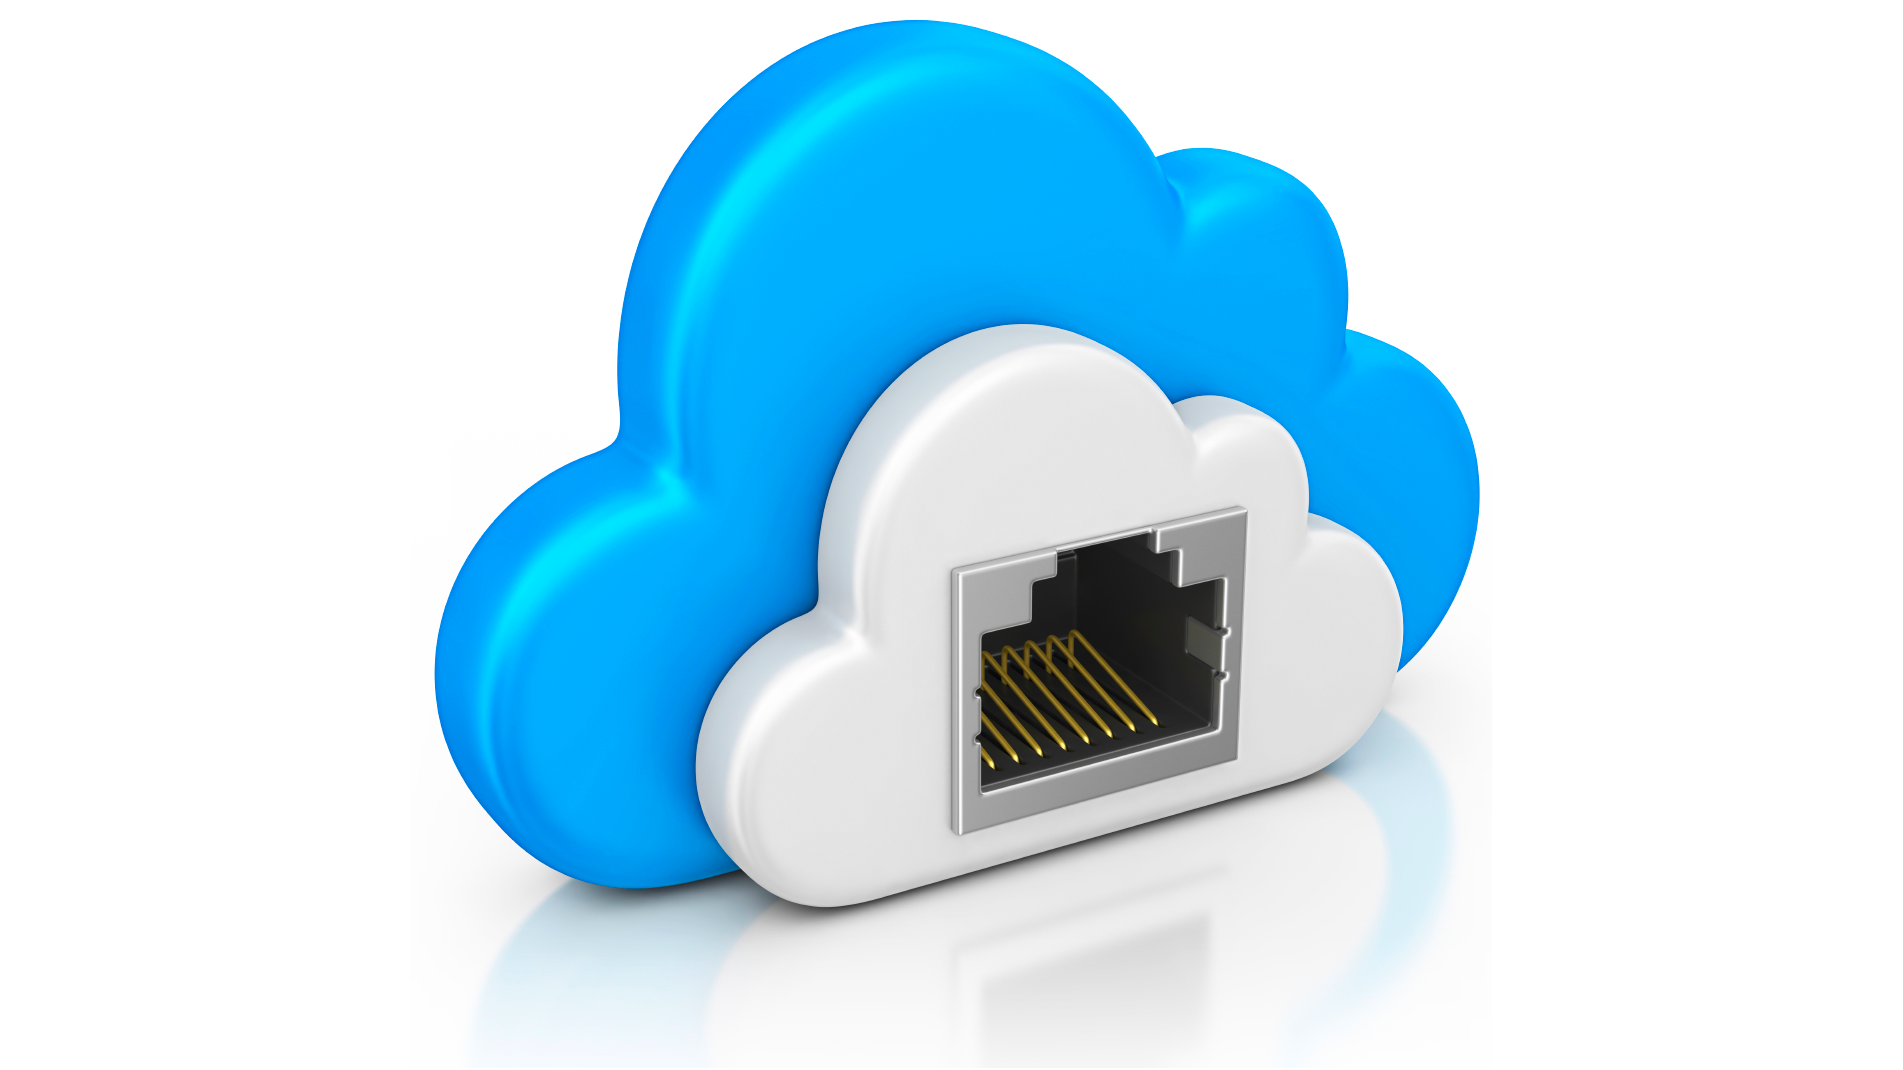
\includegraphics[width=12em]{vhg.png}
		\end{column}
										
		\begin{column}[T]{0.66\textwidth} 
										   
			\textbf{ Virtual CPE}
			\begin{itemize}
				\item Pulling Network Functions into the operator network
				\item Shared Resources, optimized dimensioning
				\item Managing $O(10^{3})$ Network Nodes is easier than $O(10^{6})$ of CPE.
			\end{itemize}
			\vspace{3mm}
			\textbf{General Approach}
			\begin{itemize}
				\item Replacing existing HG by a Layer-2 device, handling VoIP and Wifi.
				\item Current functions (eg. NAT and DHCP) are performed in the operator network
				\item The Virtual Home Gateway for extended home
			\end{itemize}
										
																																						
		\end{column}
																										
	\end{columns}
										
\end{frame}

\begin{frame}{Several Architecture are proposed by Research.}
				
	\begin{columns}[T]
		\begin{column}[T]{0.33 \textwidth} 
															
			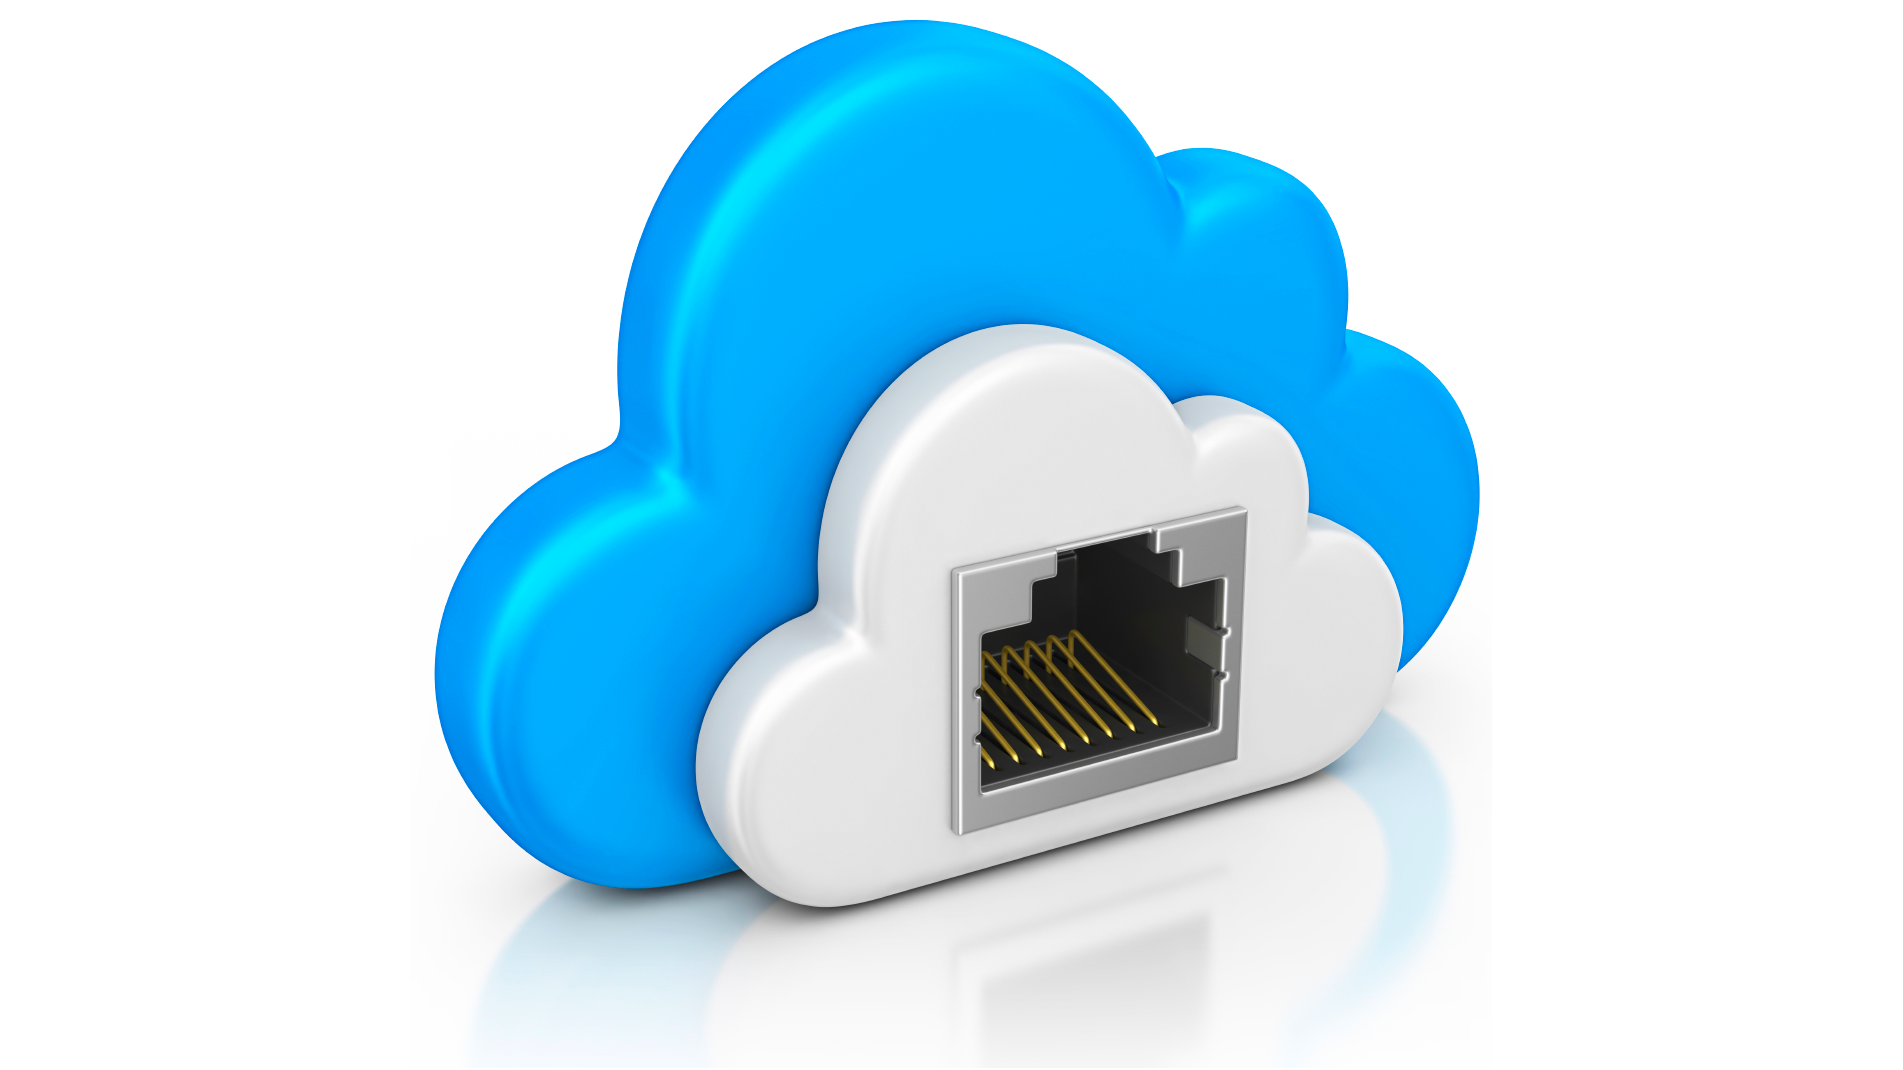
\includegraphics[width=12em]{vhg.png}
		\end{column}
										
		\begin{column}[T]{0.66\textwidth} 
										   
			\textbf{Characteristics of the different approaches}
			\begin{itemize}
				\item What do we remove from HG?
				\item Where do we operate virtualized services?
				\item How do we virtualized services?
			\end{itemize}
			\vspace{3mm}
																																						
		\end{column}
																										
	\end{columns}
				
					
\end{frame}

\begin{frame}{}
	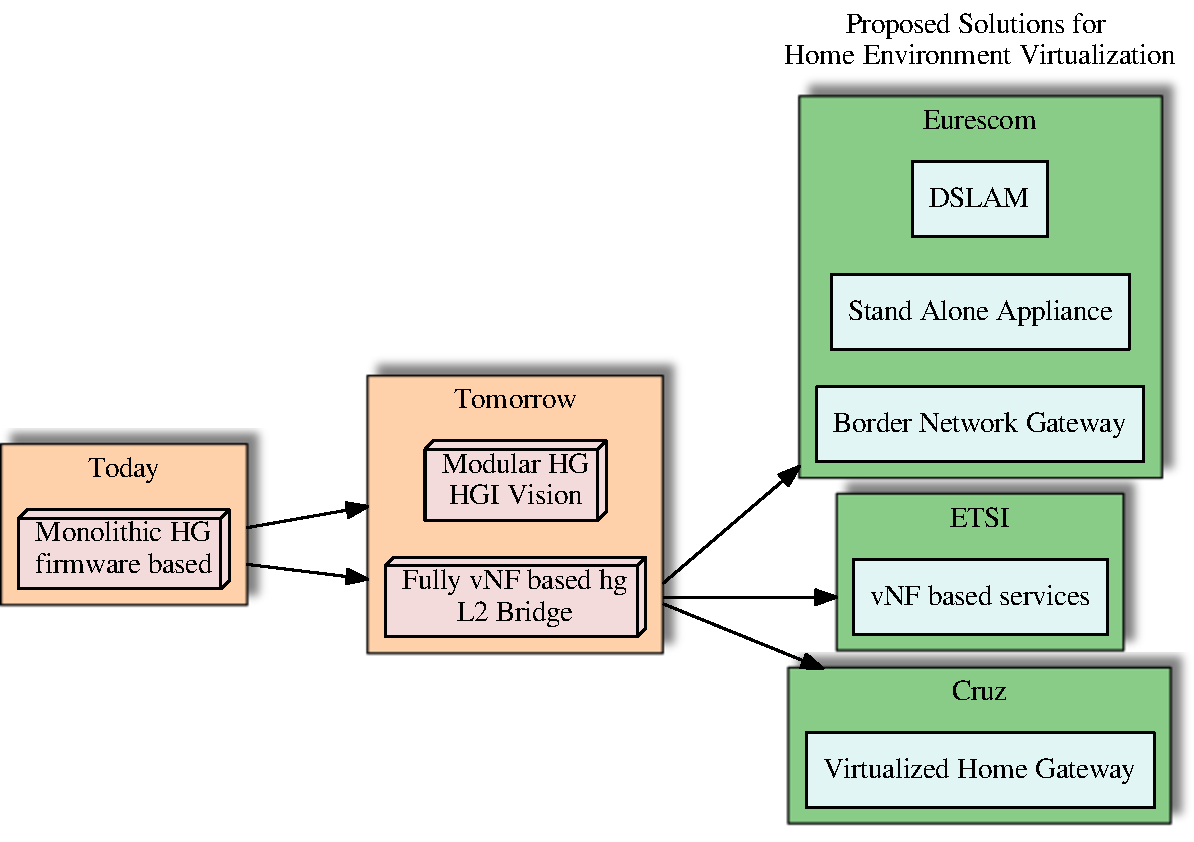
\includegraphics[width=0.9\textwidth]{vhgtrends.pdf}
\end{frame}


\begin{frame}{}
	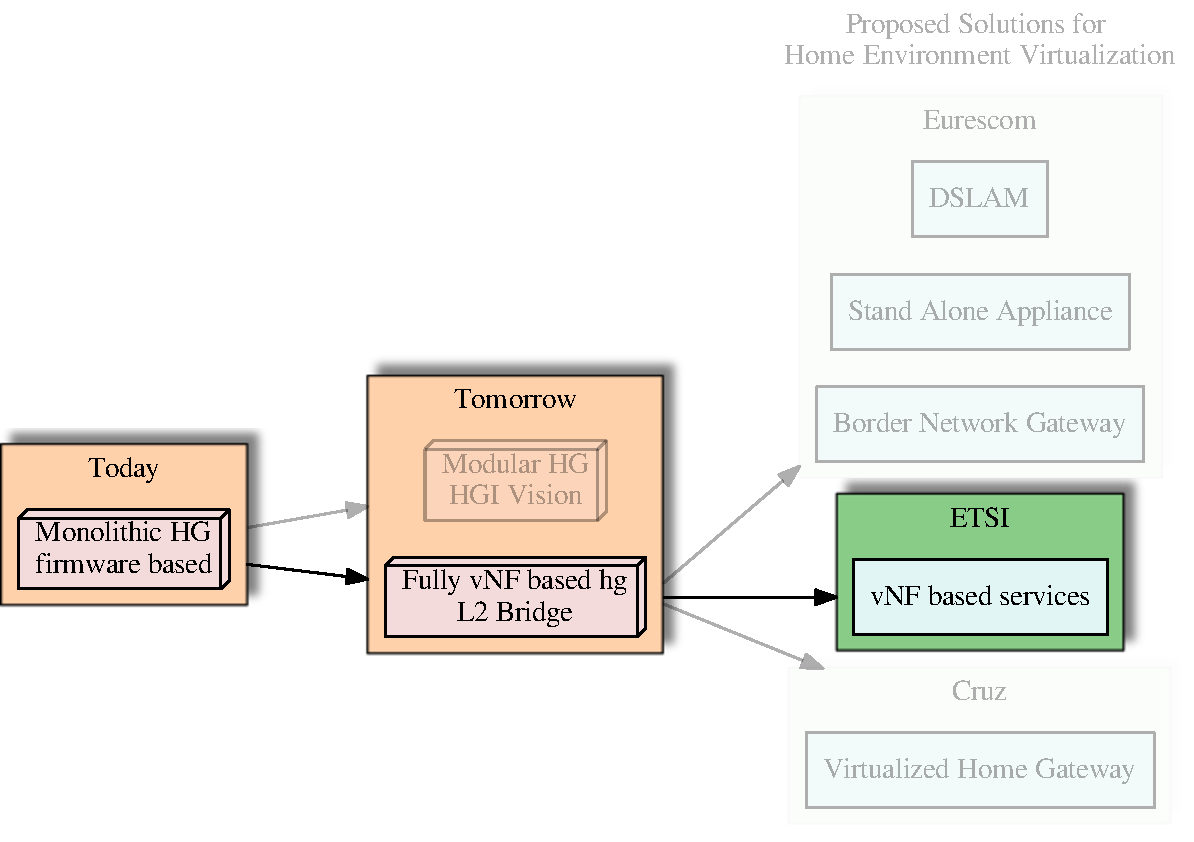
\includegraphics[width=0.9\textwidth]{vhgtrends-etsi-emphasis.pdf}
\end{frame}

\begin{frame}{}
	\begin{centering}
		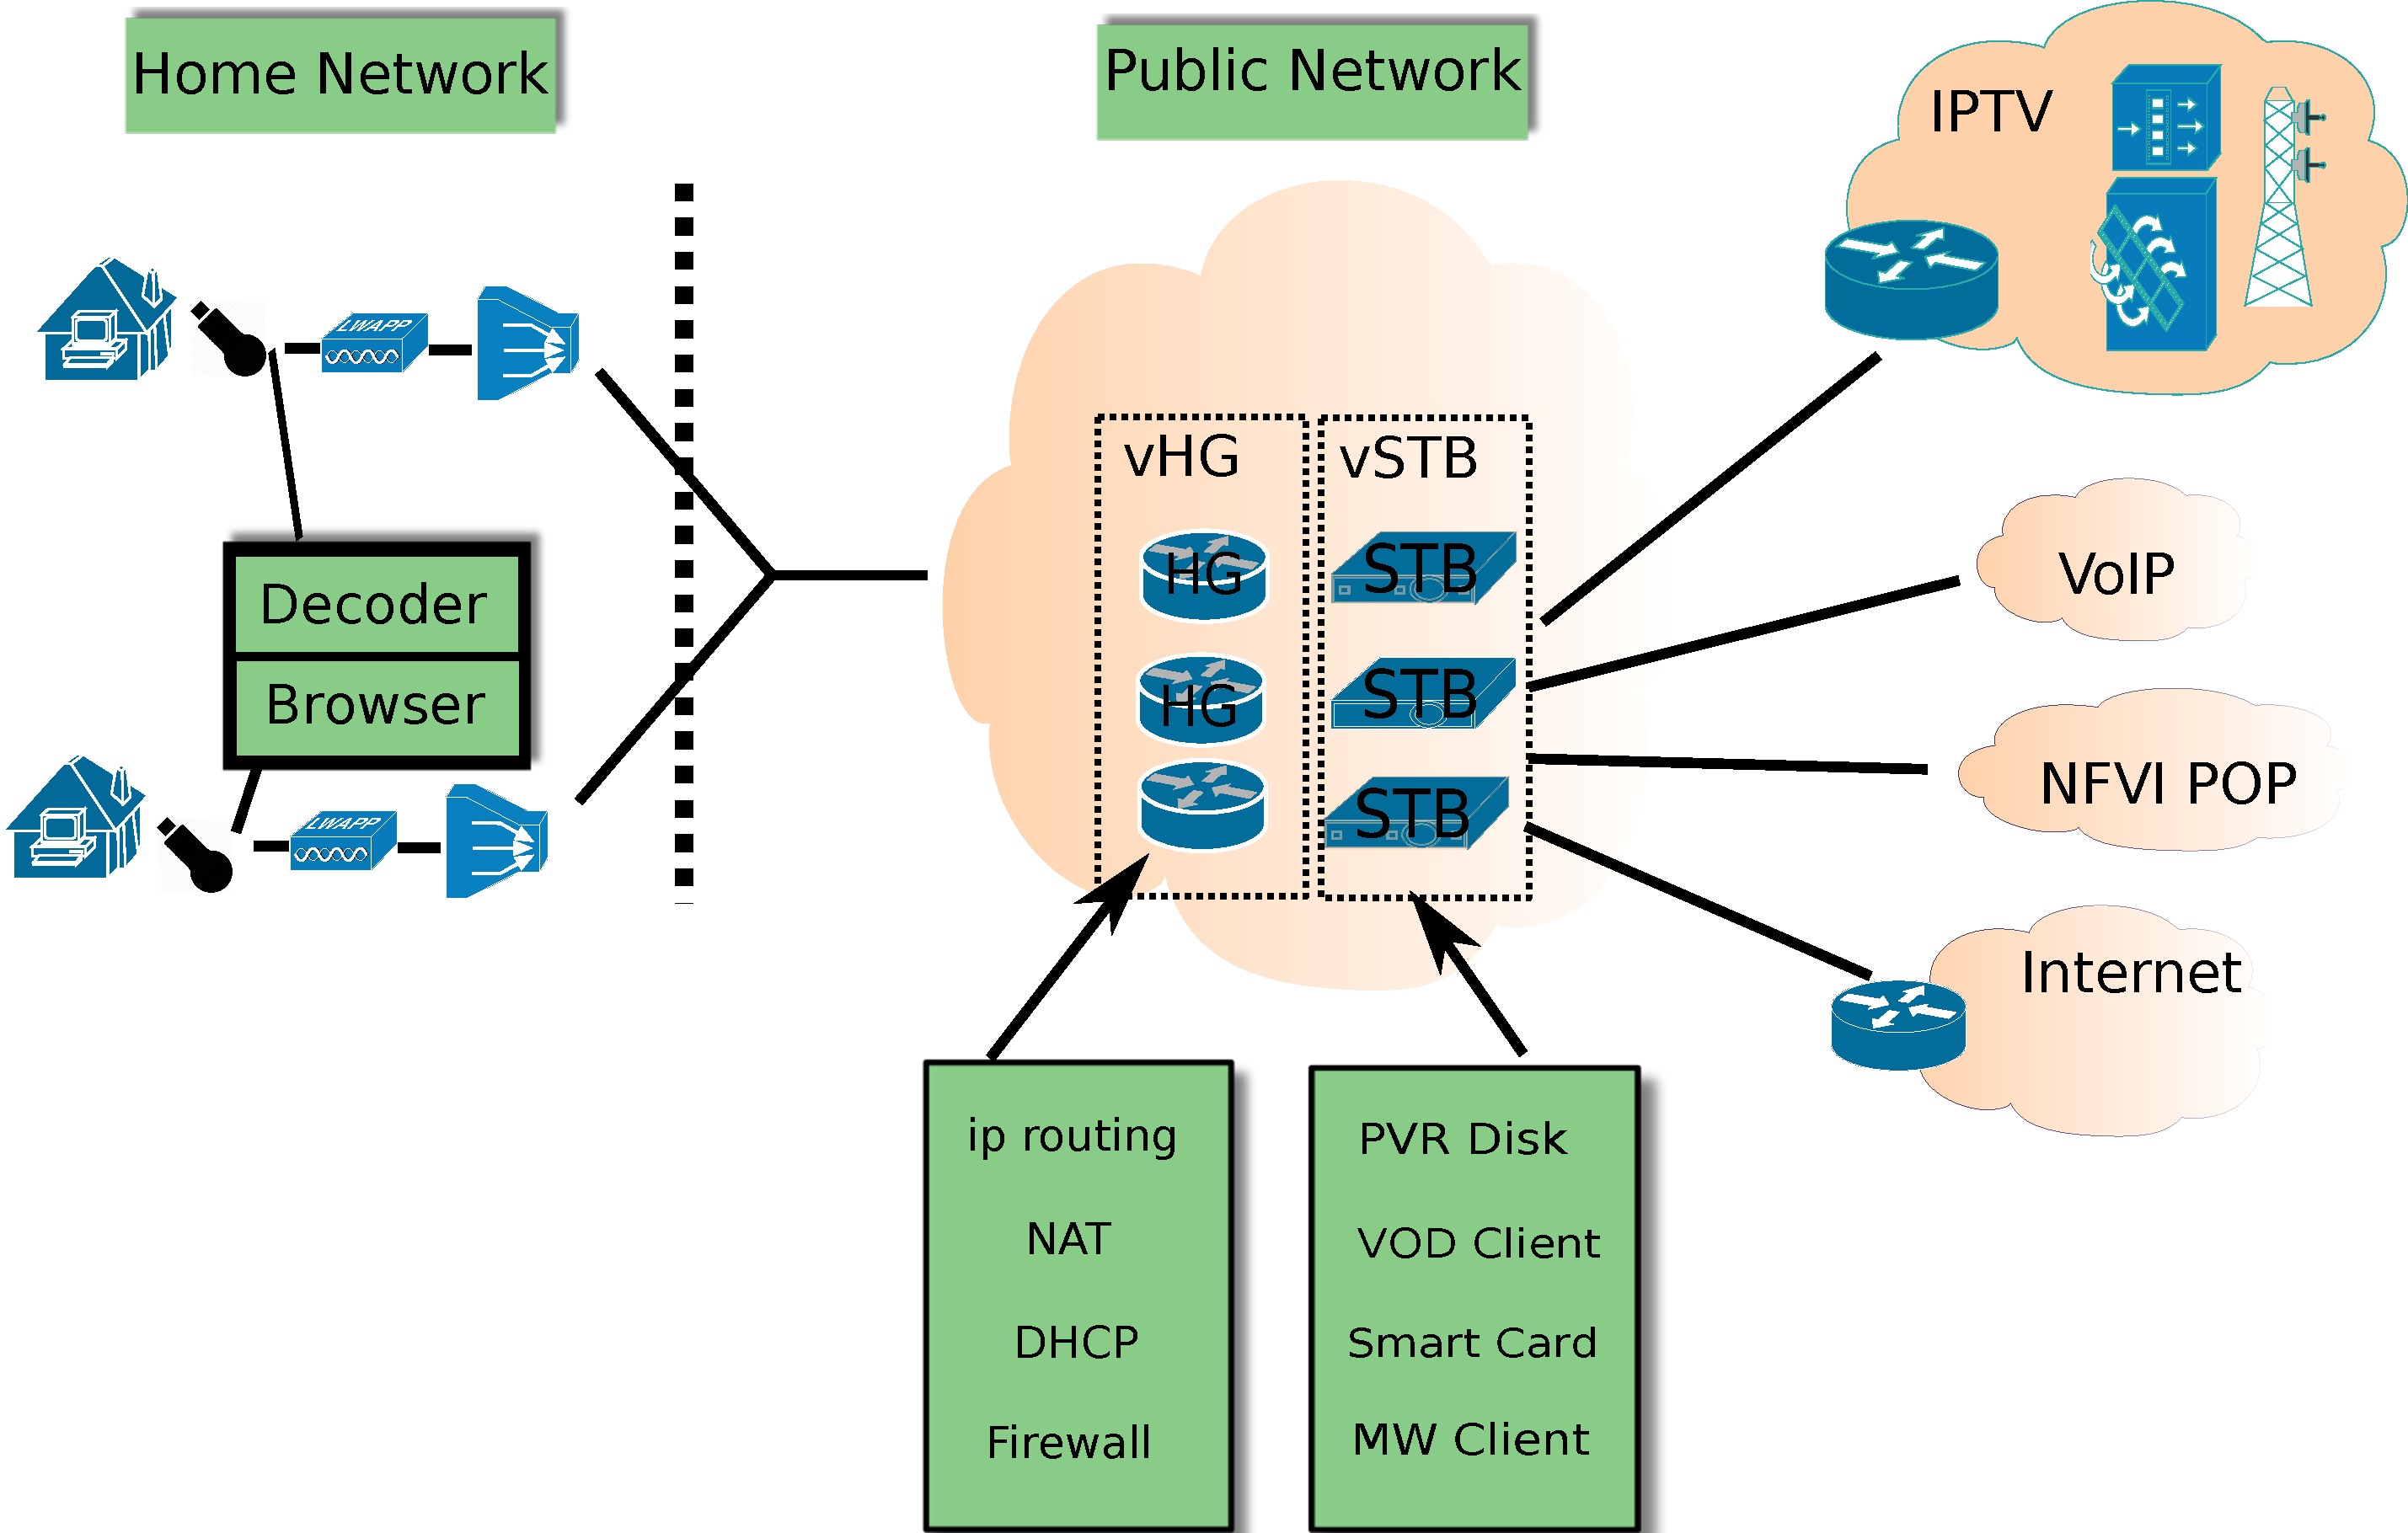
\includegraphics[width=0.9\textwidth]{etsi-virtualisation-home-env.pdf}
	\end{centering}
			
\end{frame}




\begin{frame}{Network Function Virtualization (NFV) as a building block for solving vHG issues.}
	\begin{columns}[T]
		\begin{column}[T]{0.33 \textwidth} 
			\vspace{5em}
			
\includegraphics[width=10em]{etsinfv.png}
		\end{column}
										
		\begin{column}[T]{0.66\textwidth} 
										   
			\textbf{ETSI's NFV architecture makes the operator benefits from virtualization}
			\begin{itemize}
				\item Network Functions run on commodity hardware
				\item No more middle-box vendor lock-in
				\item Multi-vendor nature boost competition and lower prices
				\item Ongoing standardization efforts
			\end{itemize}
			\vspace{3mm}
																																						
		\end{column}
																										
	\end{columns}
\end{frame}

\begin{frame}{vHG with vNF is a clean slate approach, which is an issue for migrating to this model}
	\begin{columns}[T]
		\begin{column}[T]{0.33 \textwidth} 
			\vspace{6em}
			
\includegraphics[width=10em]{etsinfv.png}
		\end{column}
										
		\begin{column}[T]{0.66\textwidth} 
										   
			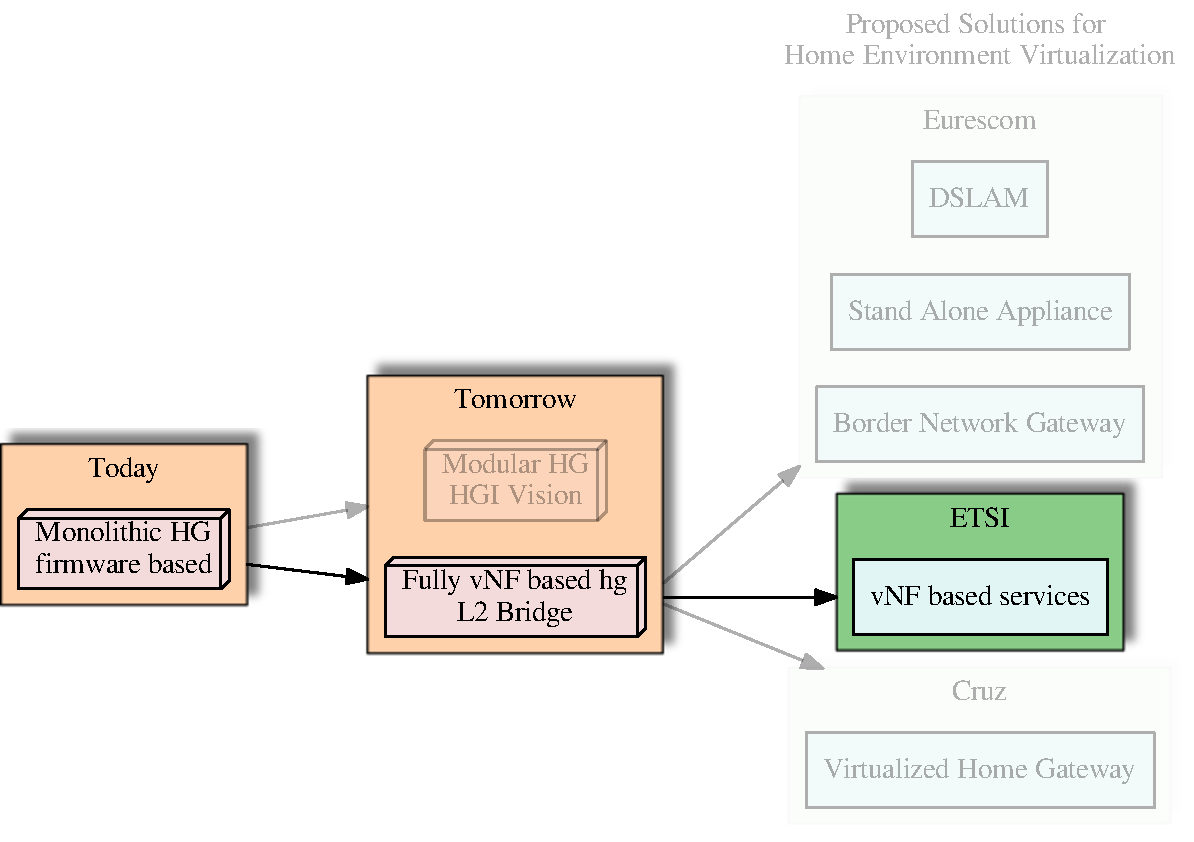
\includegraphics[width=\textwidth]{vhgtrends-etsi-emphasis.pdf}
																																						
		\end{column}
																										
	\end{columns}
\end{frame}





\setbeamercolor{frametitle}{bg=applegreen}
\setbeamercolor{frametitle right}{bg=applegreen!90}
\setbeamercolor{footline left}{bg=applegreen}
\setbeamercolor{section in head/foot}{fg=black, bg=applegreen}
\setbeamercolor{title in head/foot}{fg=black, bg=applegreenpale}


\begin{frame}{vHG with vNF is a clean slate approach, which is an issue for migrating to this model}
	\begin{columns}[T]
		\begin{column}[T]{0.33 \textwidth} 
			\vspace{6em}
			
\includegraphics[width=10em]{etsinfv.png}
		\end{column}
										
		\begin{column}[T]{0.66\textwidth} 
										   
			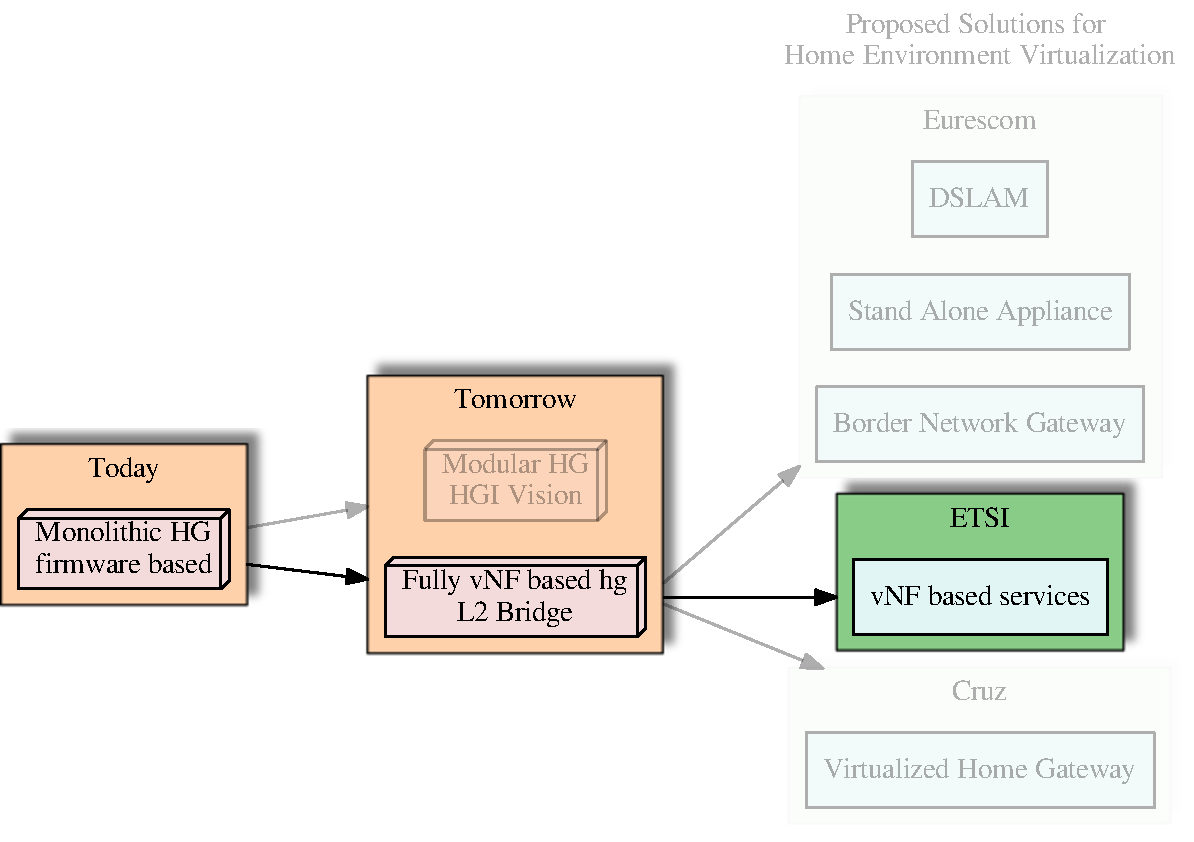
\includegraphics[width=\textwidth]{vhgtrends-etsi-emphasis.pdf}
																																						
		\end{column}
																										
	\end{columns}
	\setbeamercolor{block title}{bg=applegreen}
	\begin{textblock*}{8cm}(3cm,0.4\textheight)
		\begin{block}{}
			\textbf{ This is where our contribution helps }
			\begin{itemize}
				\item We propose a way to migrate progressively to this final model
				\item We want to start benefiting from NFV as soon as possible
				\item We leverage standards as much as possible
			\end{itemize}
		\end{block}
	\end{textblock*}		
\end{frame}


\begin{frame}{Our contribution eases the migration to vHG}
	
	\begin{flushleft}	
		\textbf{We introduce de Surrogate vNF (SvNF) Concept}
		\begin{itemize}
			\item 1. We start from a modular HGI OSGi-capable HG
			\item 2. We deploy a SvNF module as a drop-in replacement for a HG native function or as a new service
			\item 3. The SvNF delegates any significant operation to a remote vNF
			\item 4. vNFs can be used in both the modular HG or in NVF-Based HG
		\end{itemize}
	\end{flushleft}
	\centering
	\framebox{	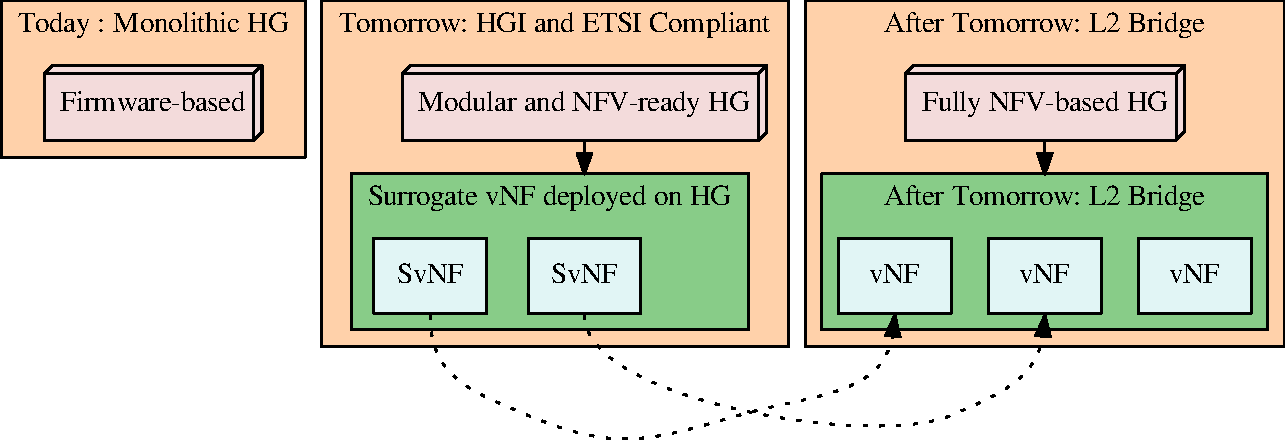
\includegraphics[width=25em]{migrationPath.pdf}}\\
			
\end{frame}

\begin{frame}{Example of SvNF+vNF}
	\begin{flushleft}	
		\textbf{Parental Control}
		\begin{itemize}
			\item The service allows or denies the traffic (control plane), depending on schedule
			\item The service detects on-line gaming traffic and applies a daily quotas
			\item The service allow remote control and cross-devices policy
		\end{itemize}
	\end{flushleft}
	\vspace{2em}
	\centering
	\framebox{	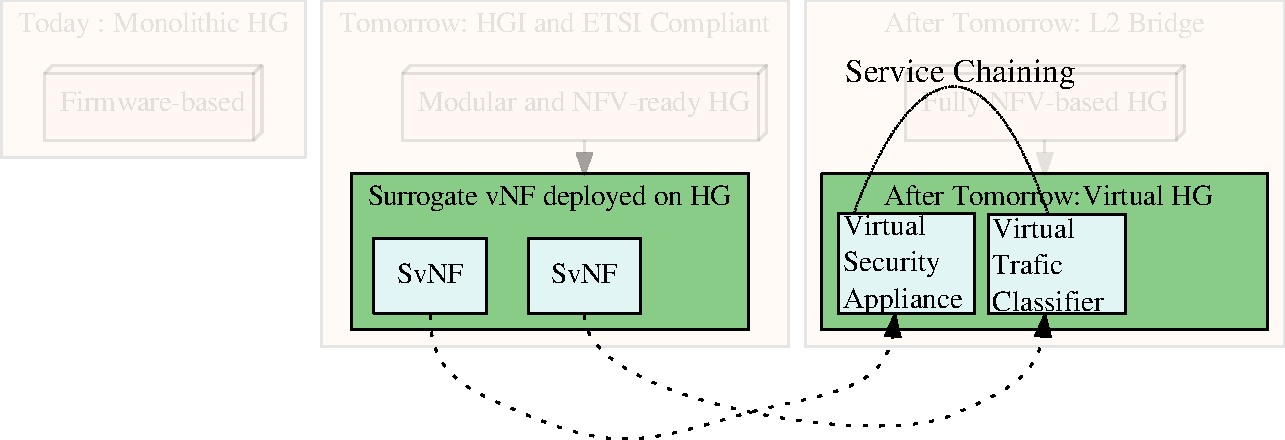
\includegraphics[width=25em]{migrationPath-example.pdf}}\\
			
\end{frame}


\begin{frame}{SvNF Life-cycle respects OSGi standard, while adding new semantics to fit Network Functions operations}
	\begin{flushleft}	
		\textbf{Relation with OSGi life-cycle}
		\begin{itemize}
			\item We consider software and network dependencies
			\item If the vNF is not available, the module is not loaded
			\item and we fall back on legacy mode
		\end{itemize}
	\end{flushleft}
	\vspace{2em}
	\centering
	\framebox{	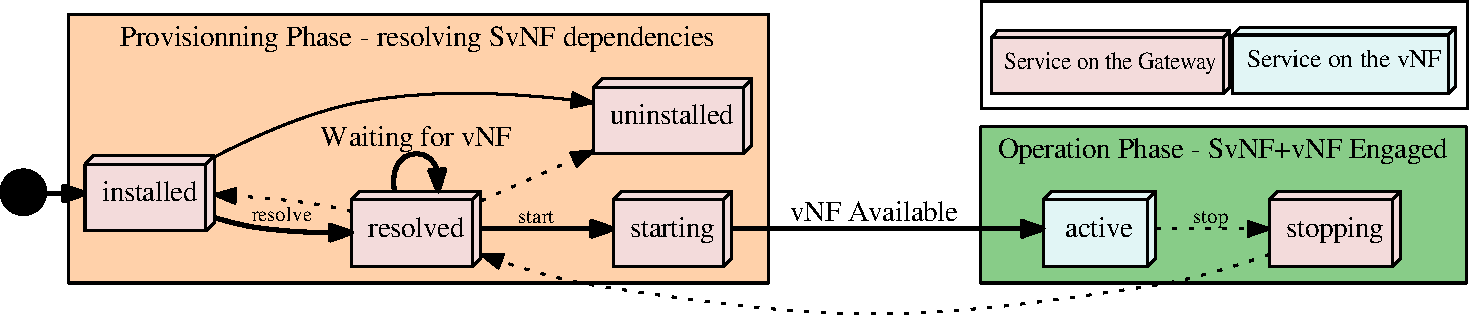
\includegraphics[width=25em]{osgi.pdf}}\\
\end{frame}


\begin{frame}{Feasibility Study illustrated by a Content Delivery Use case}
	\begin{columns}[T]
		\begin{column}[T]{0.33 \textwidth} 
			\vspace{1.5cm}
			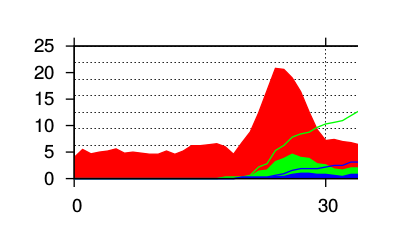
\includegraphics[width=12em]{results.png}
		\end{column}
										
		\begin{column}[T]{0.66\textwidth} 
										   
			\textbf{Rationale}
			\begin{itemize}
				\item We focus on pushing a new service to the HG using the SvNF+vNF approach
				\item It uses several vNF chained to offer a content distribution service
				\item More basic NF (NAT, DHCP) are feasible with the same pattern
			\end{itemize}
			\vspace{3mm}
			\textbf{Topic we address in the evaluation}
			\begin{itemize}
				\item How does the SvNF fits on the HG?
				\item What is the value brought by the overall service?
				\item How do we optimize service operations?
			\end{itemize}
		\end{column}
																										
	\end{columns}
								
\end{frame}


\begin{frame}{}
	\centering
	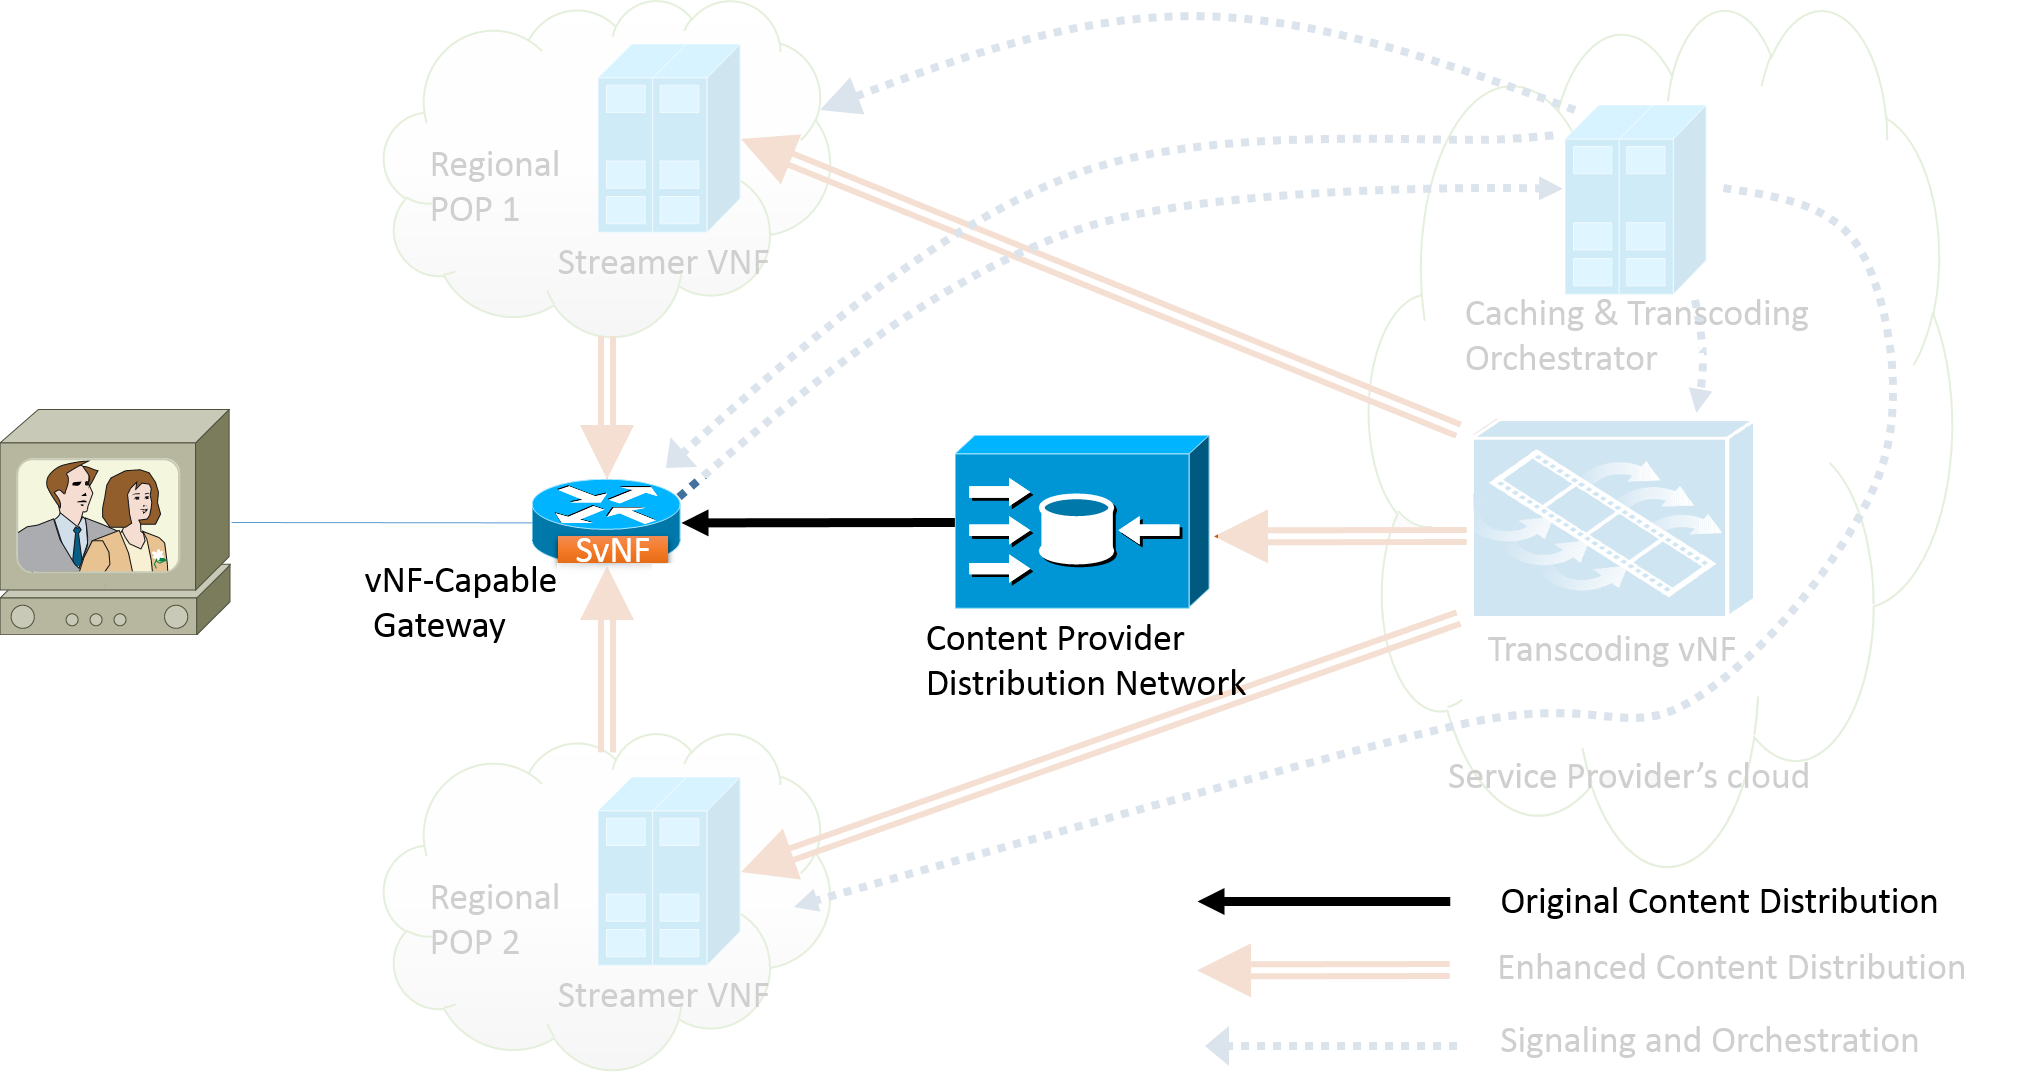
\includegraphics[width=0.95\linewidth]{highleveldesign1.png}
	\vspace{2em}
	\setbeamercolor{block title}{bg=applegreen}
	\begin{block}{}
		A User consumes media on a screen, data is received on her HG from the Content Provider (CP) Distribution Network
	\end{block}
	
\end{frame}

\begin{frame}{}
	\centering
	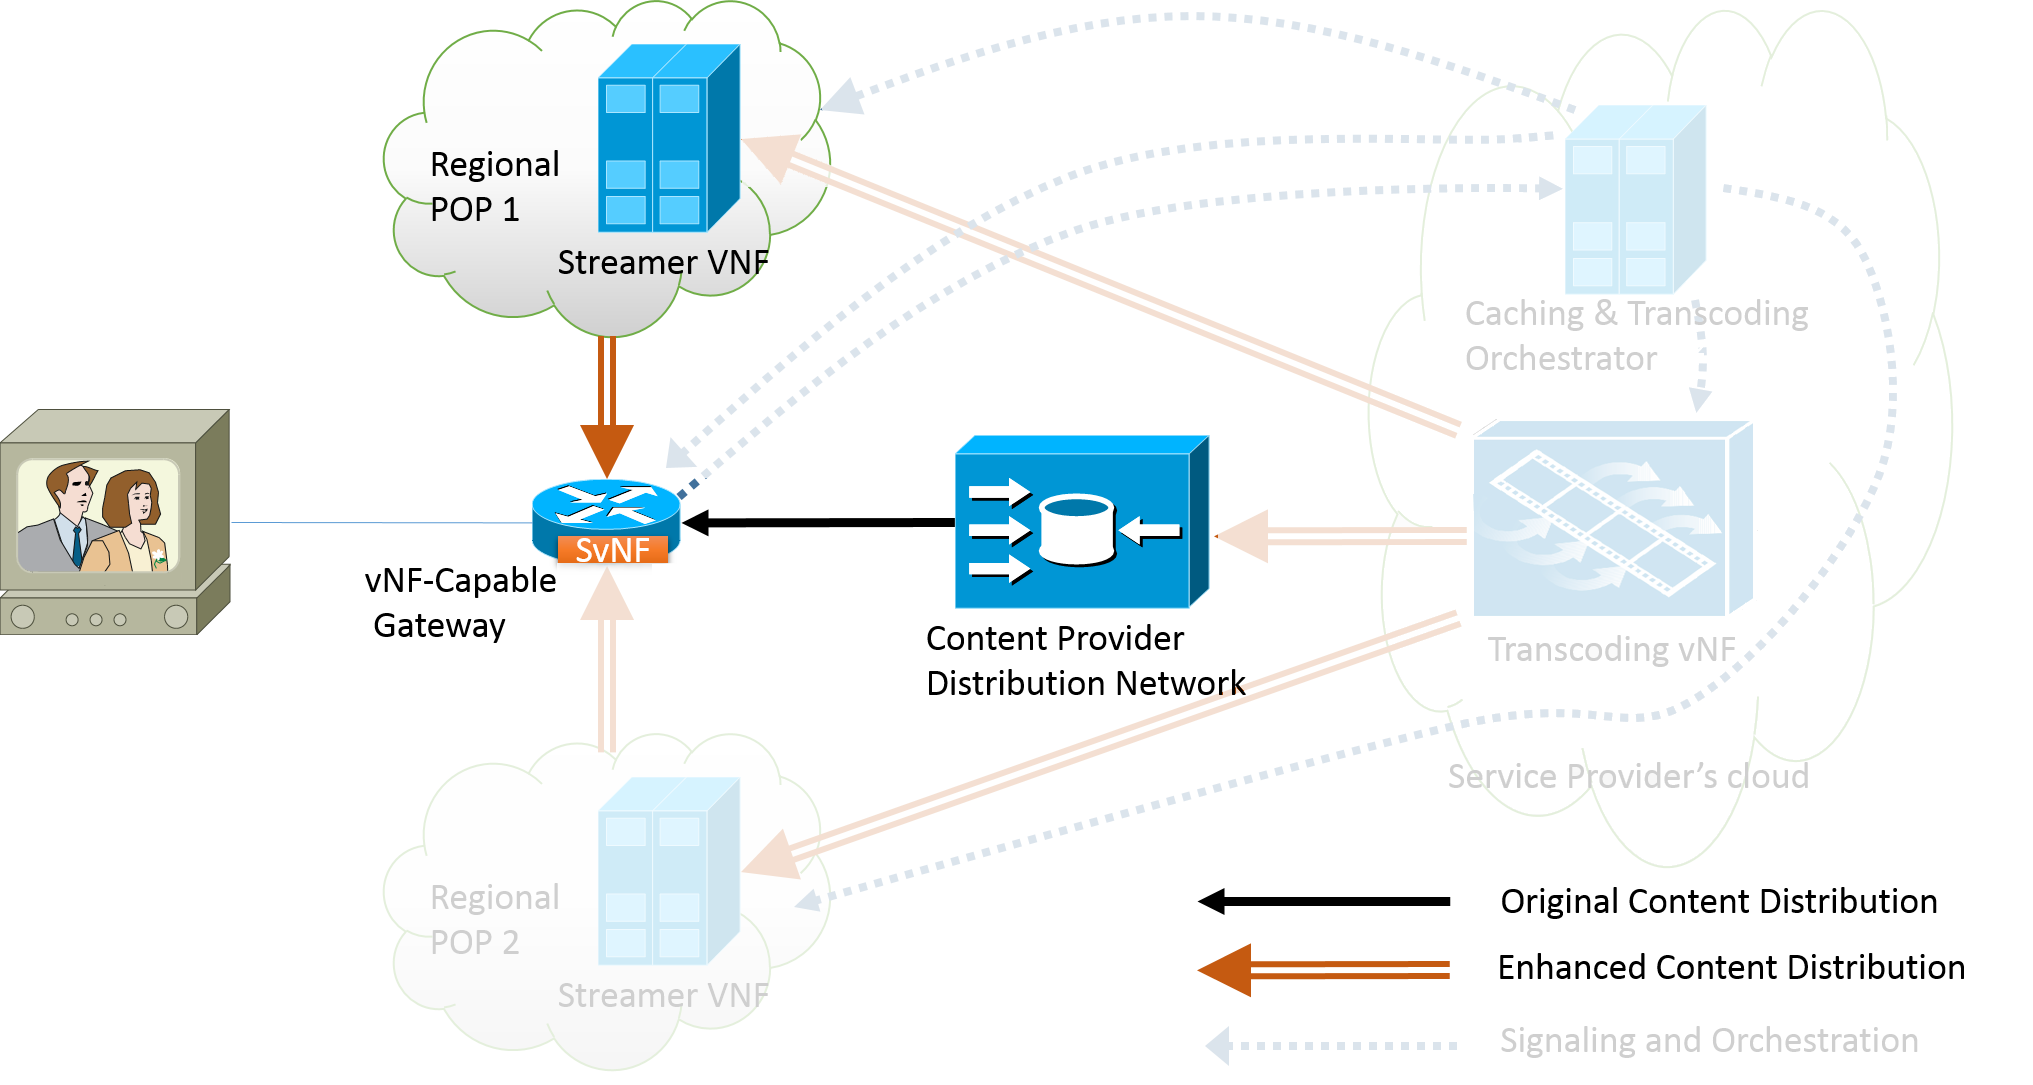
\includegraphics[width=0.95\linewidth]{highleveldesign2.png}
	\vspace{1em}
	\setbeamercolor{block title}{bg=applegreen}
	\begin{block}{}
		Media data is usually hosted on the CP network, but it can also be hosted in a Point Of Presence, a micro data-center close to the user belonging to the SP network. The Streamer vNF is responsible for delivery.
	\end{block}
\end{frame}

\begin{frame}{}
	\centering
	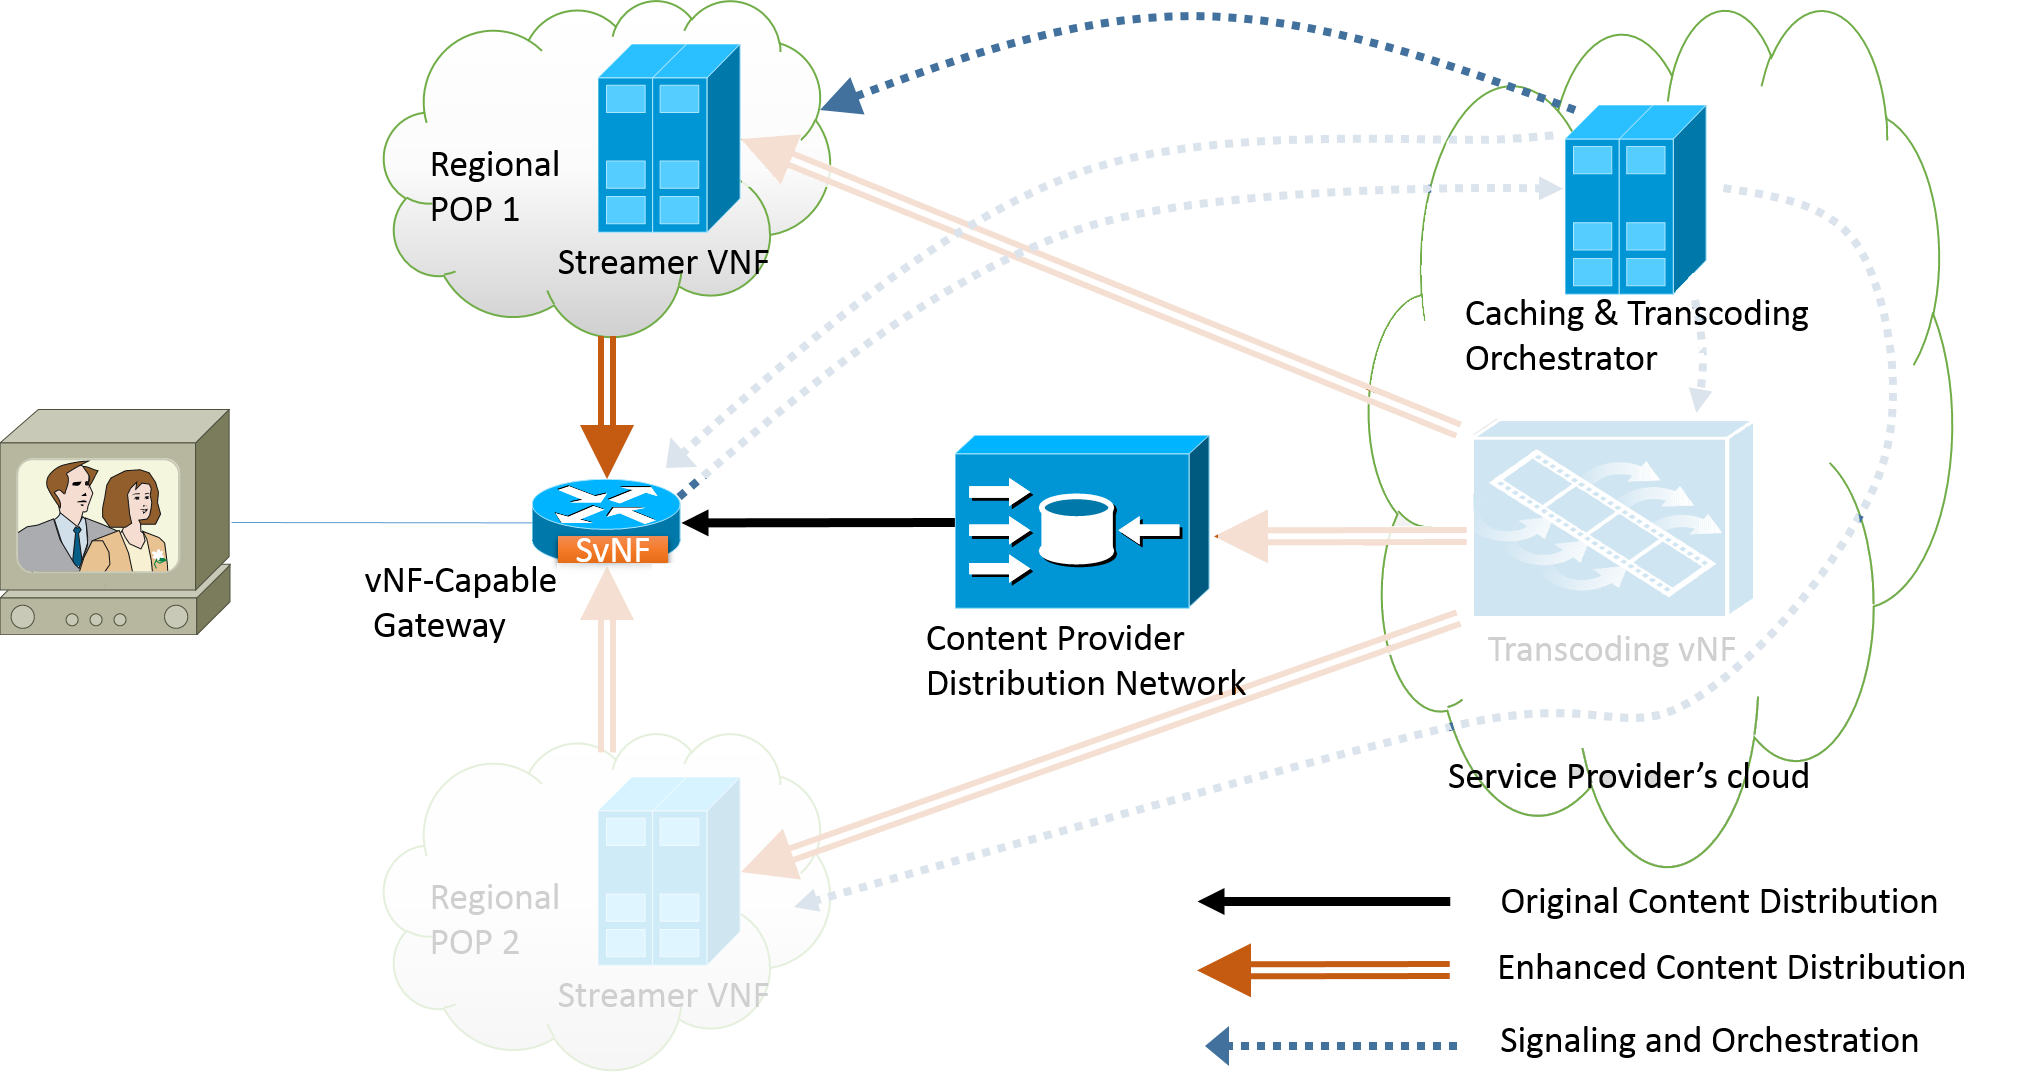
\includegraphics[width=0.95\linewidth]{highleveldesign3.png}
	\vspace{2em}
	\setbeamercolor{block title}{bg=applegreen}
	\begin{block}{}
		POP and Streamer vNF are provisioning is the responsibility of a Caching Orchestrator, placed in the SP public cloud.
	\end{block}
\end{frame}

\begin{frame}{}
	\centering
	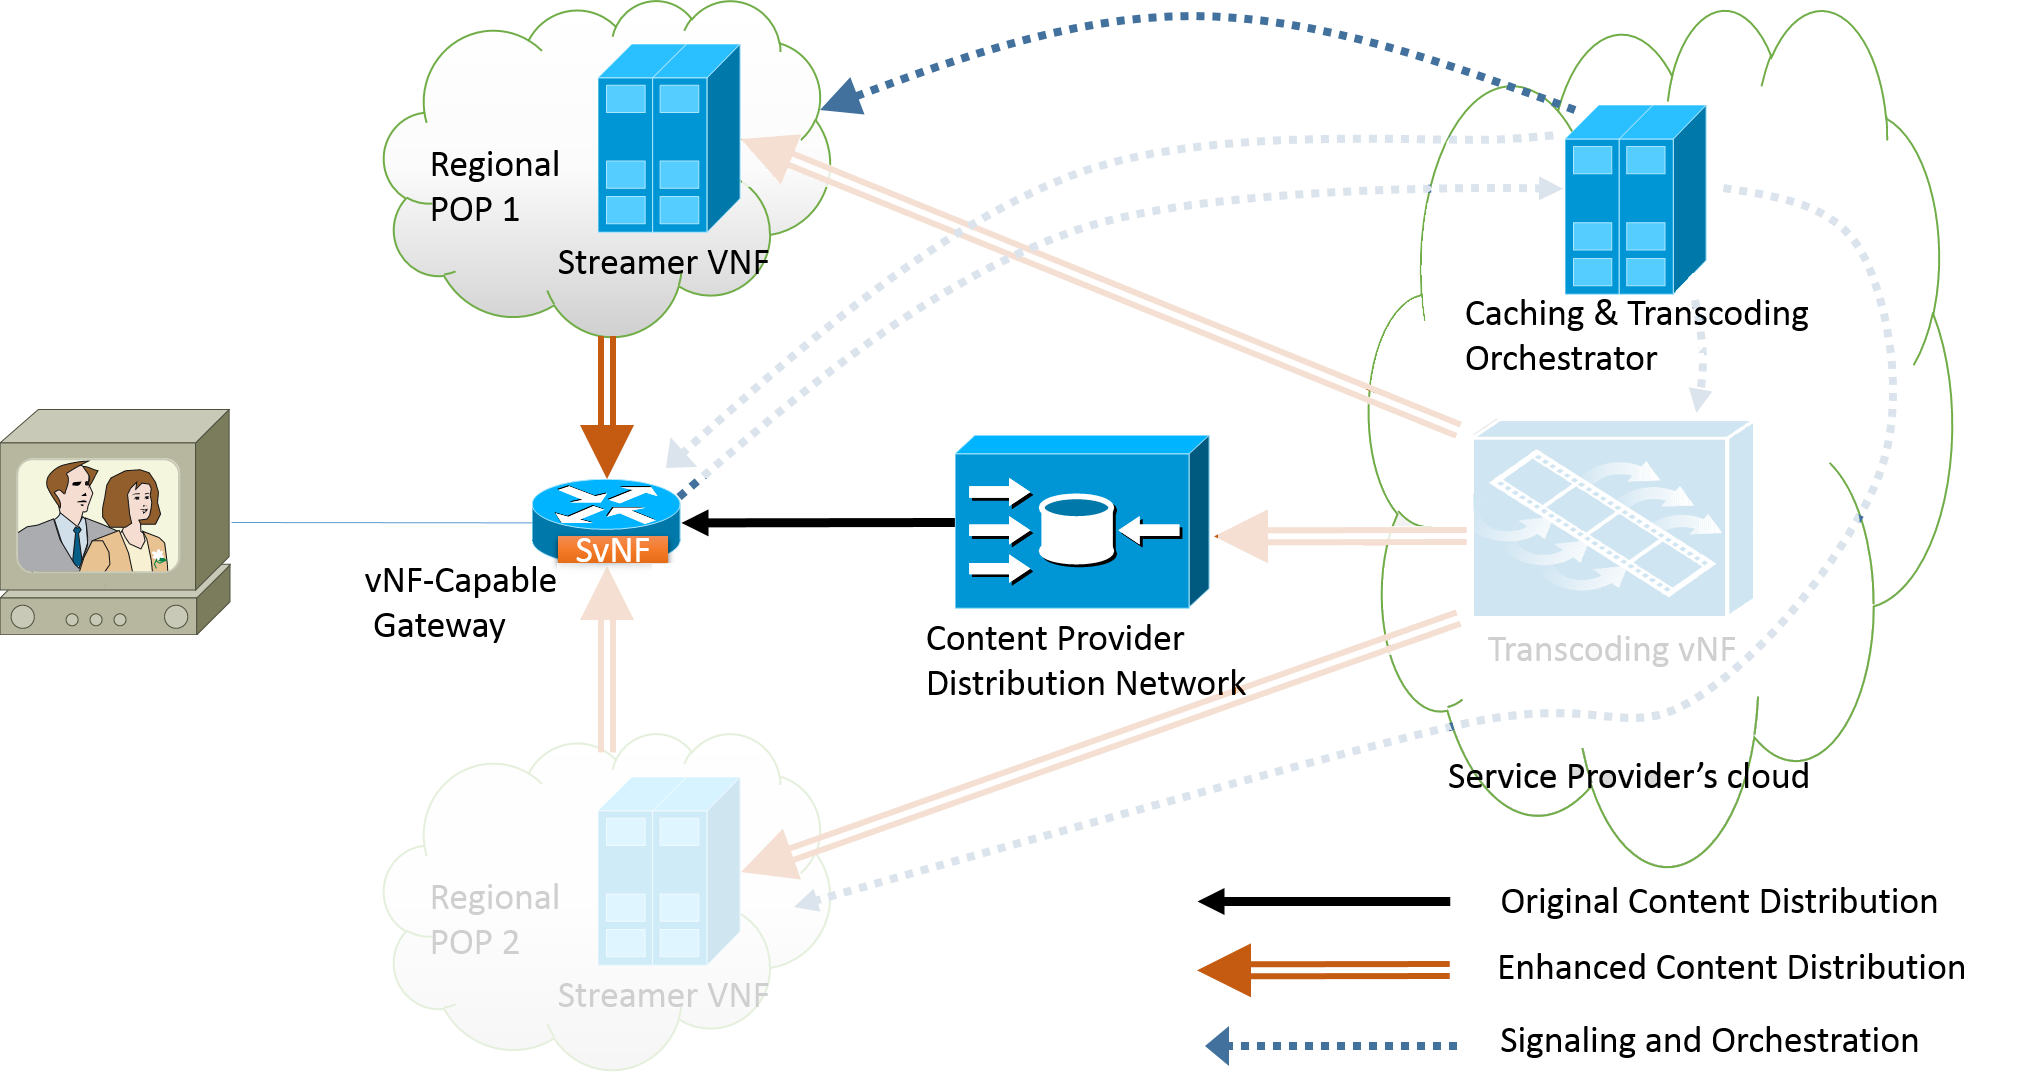
\includegraphics[width=0.95\linewidth]{highleveldesign3.png}
	\vspace{2em}
	\setbeamercolor{block title}{bg=applegreen}
	\begin{block}{}
		POP and Streamer vNF are provisioning is the responsibility of a Caching Orchestrator, placed in the SP public cloud.
	\end{block}
		\begin{textblock*}{8cm}(3cm,0.4\textheight)
		\begin{alertblock}{}
			\textbf{ How does we forward user request to POP? }
			\begin{itemize}
				\item The traditional approach is to use DNS-Based Request routing or IP anycast
				\item Research suggest using Software Defined Networks (SDN) for future deployments
				\item We take this approach, by allowing the SvNF to route the user request to a particular POP.
			\end{itemize}
		\end{alertblock}
	\end{textblock*}		
\end{frame}

\begin{frame}{}
	\centering
	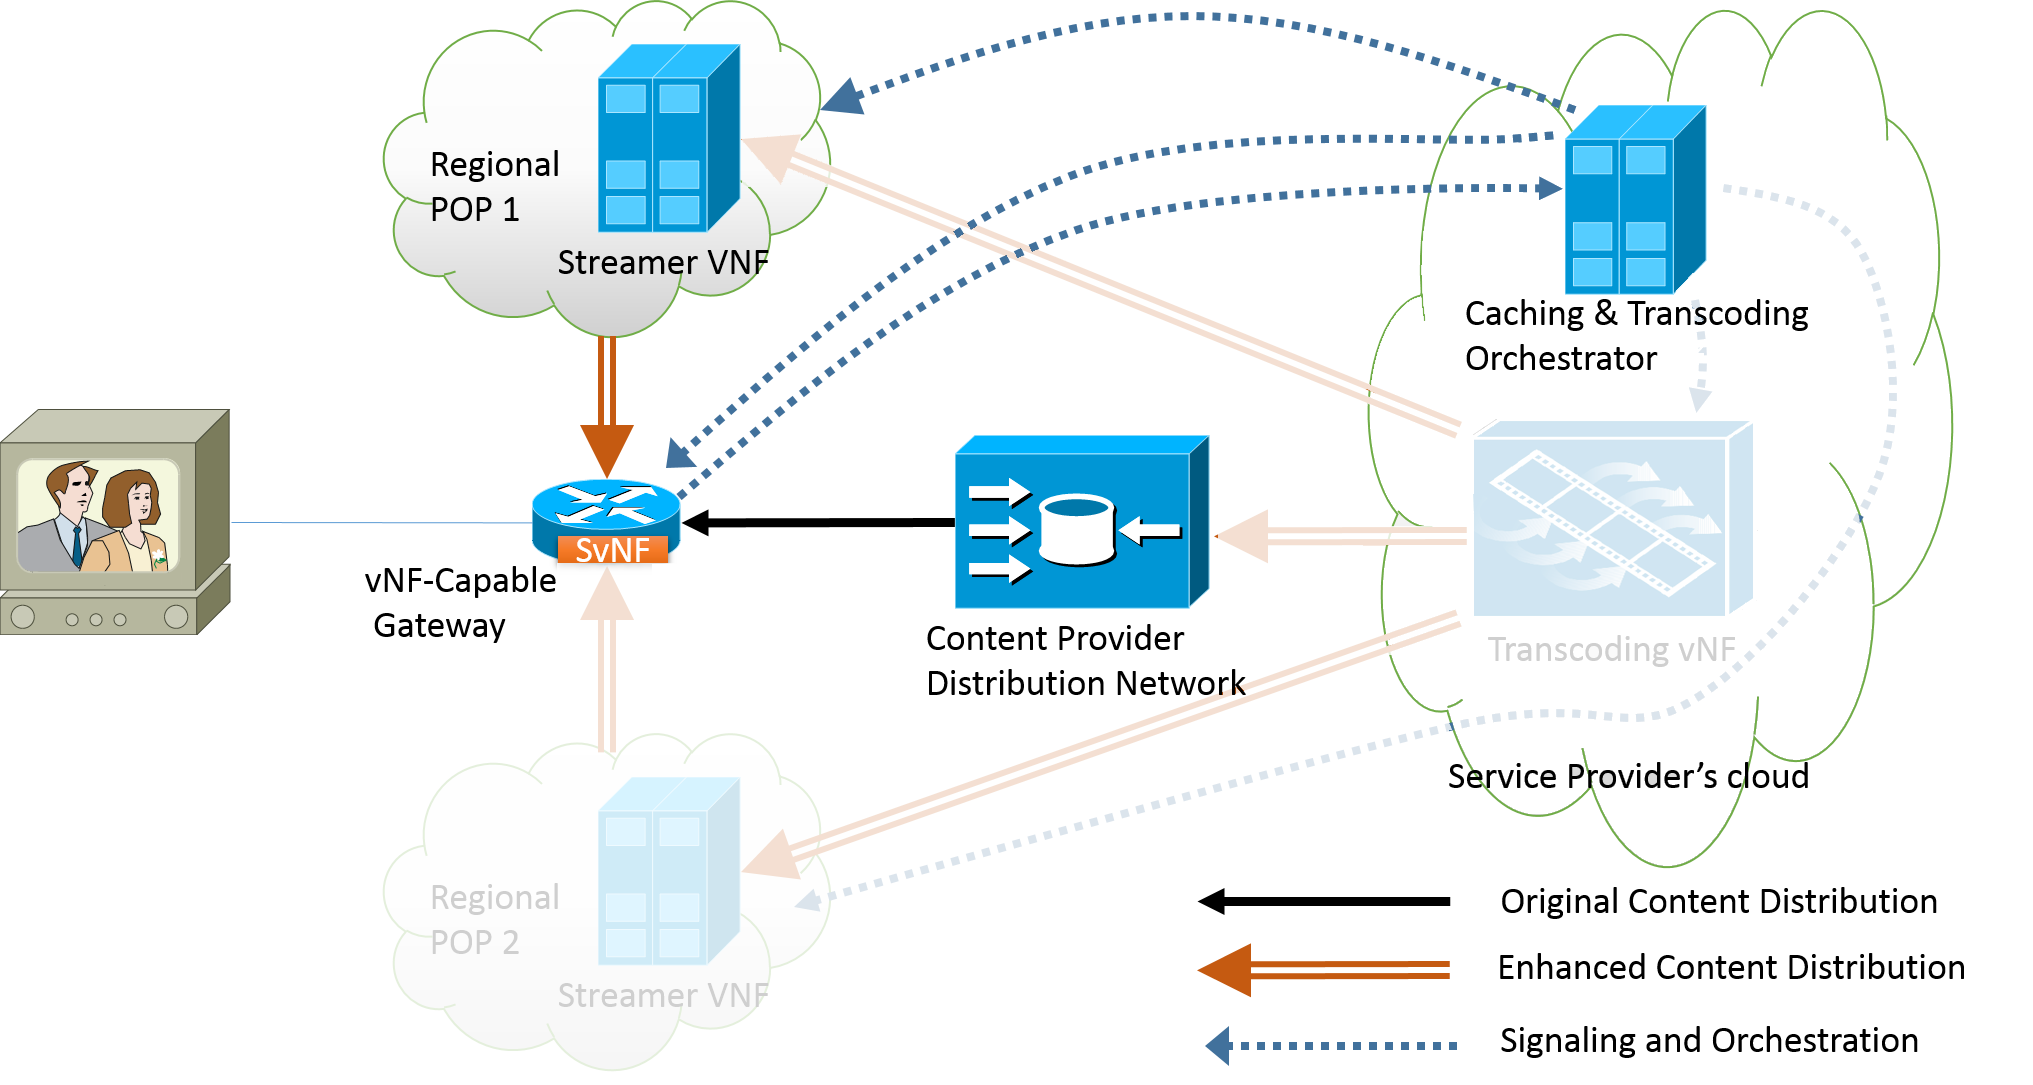
\includegraphics[width=0.95\linewidth]{highleveldesign4.png}
	\vspace{1em}
	\setbeamercolor{block title}{bg=applegreen}
	\begin{block}{}
		Caching Orchestrator deploys routing rules to SvNF. SvNF is an HTTP proxy, which allows fine-grained rules to be deployed (domain based, IP based or even content-type based).
	\end{block}
\end{frame}


\begin{frame}{}
	\centering
	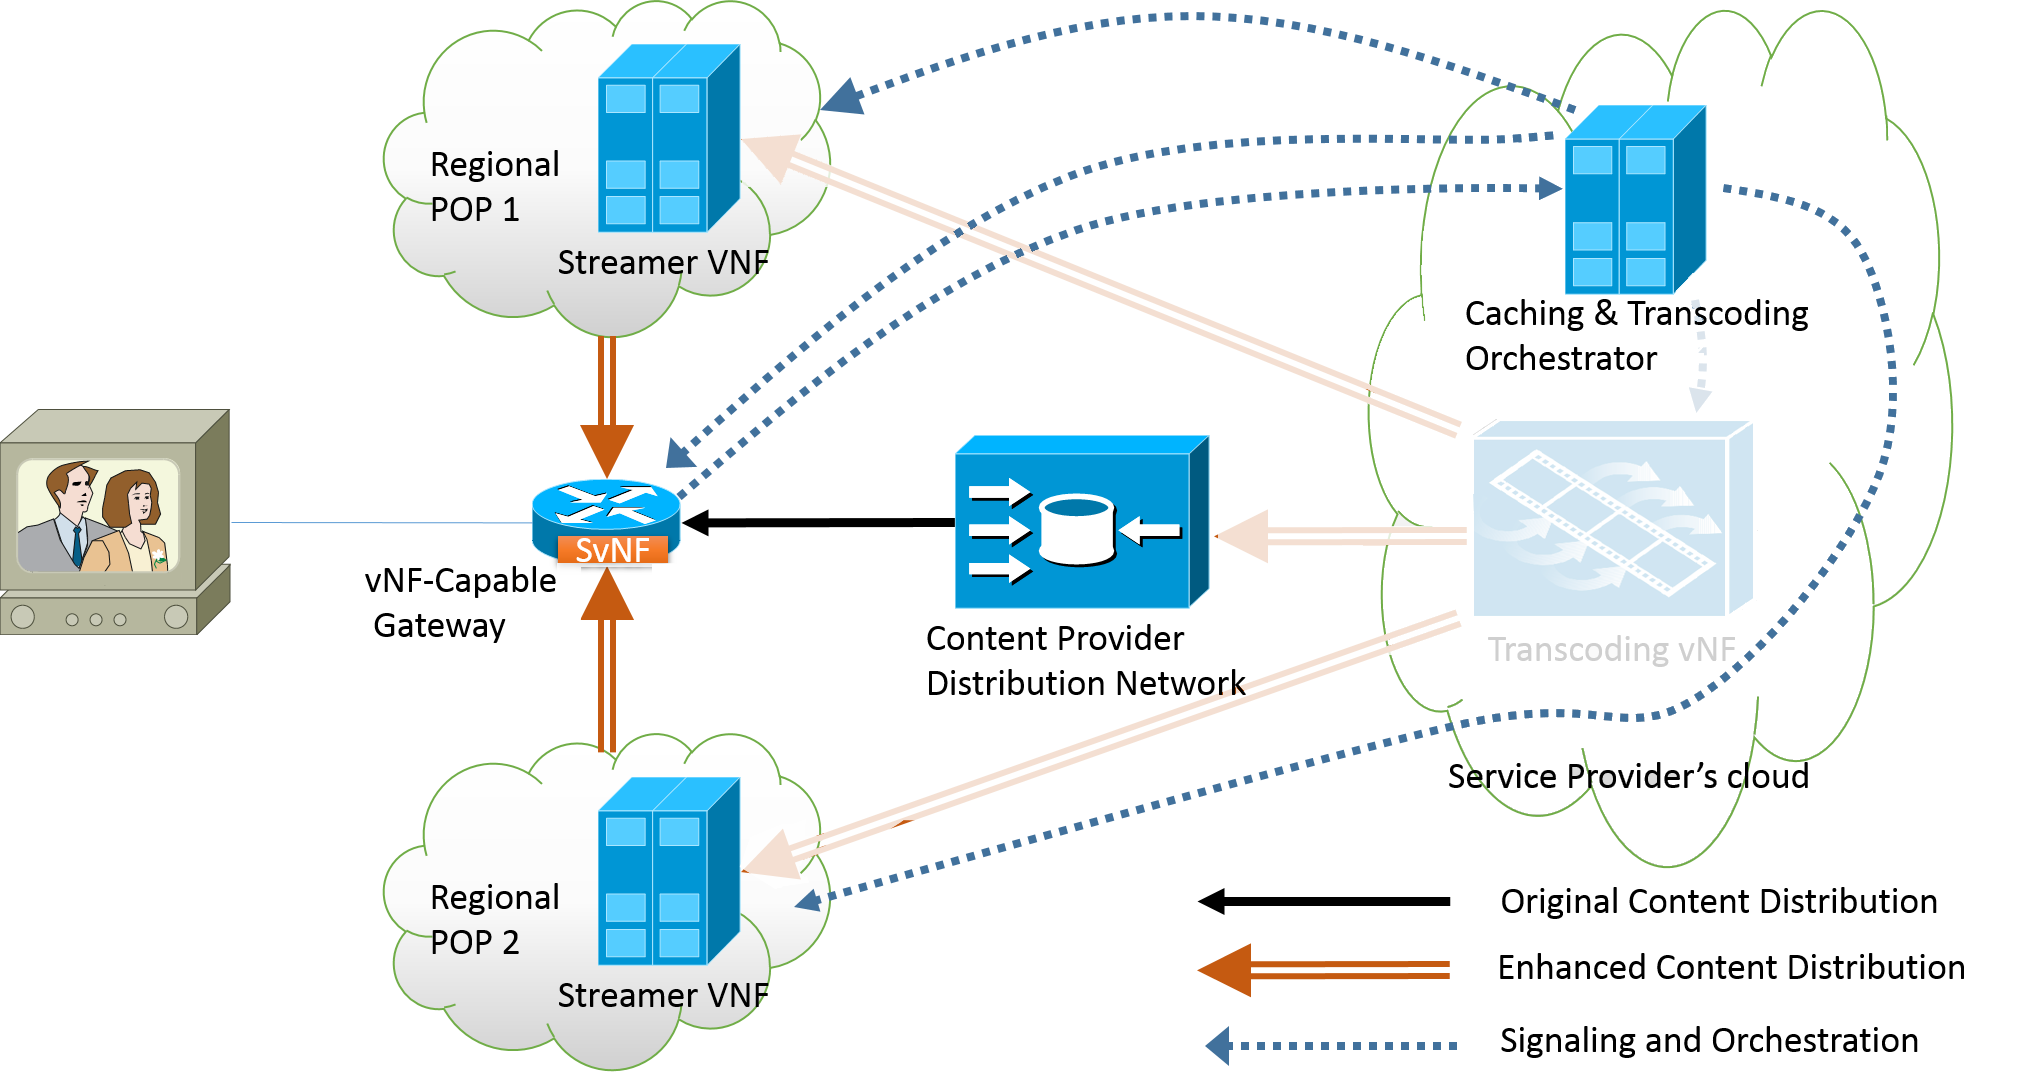
\includegraphics[width=0.95\linewidth]{highleveldesign5.png}
		\vspace{1em}
		\setbeamercolor{block title}{bg=applegreen}
	\begin{block}{}
		SvNF collaborates with the Caching Orchestrator to provide data usage statistics that can be used to provision precisely the POPs where data is needed.
	\end{block}

\end{frame}


\begin{frame}{}
	\centering
	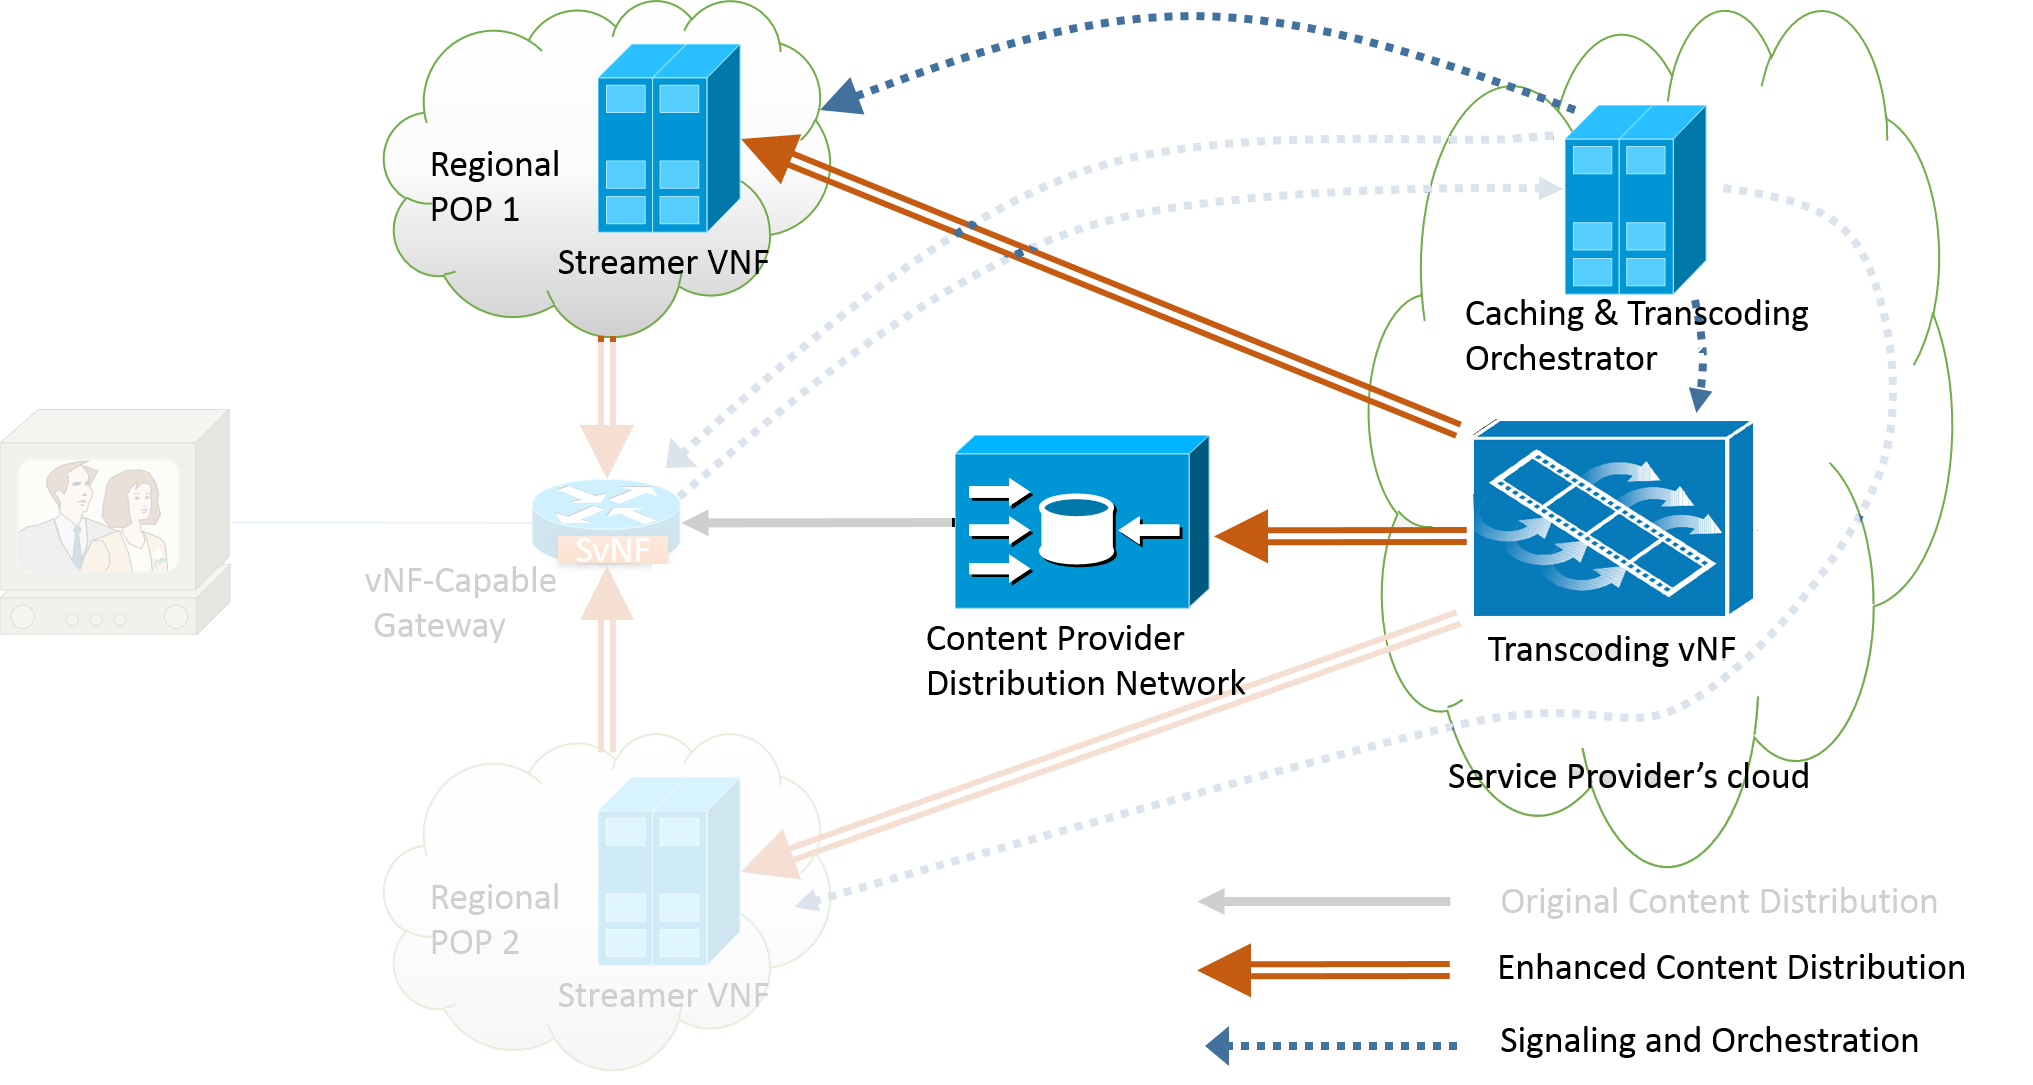
\includegraphics[width=0.95\linewidth]{highleveldesign6.png}
	\vspace{1em}
	\setbeamercolor{block title}{bg=applegreen}
	\begin{block}{}
		The vNF approach allows the Service Provider Delivery Network to handle heavy lifting operations on media, like Transcoding. New transcoding algorithms can be easily pushed to the SP cloud.
	\end{block}
\end{frame}


\begin{frame}{}
	\centering
	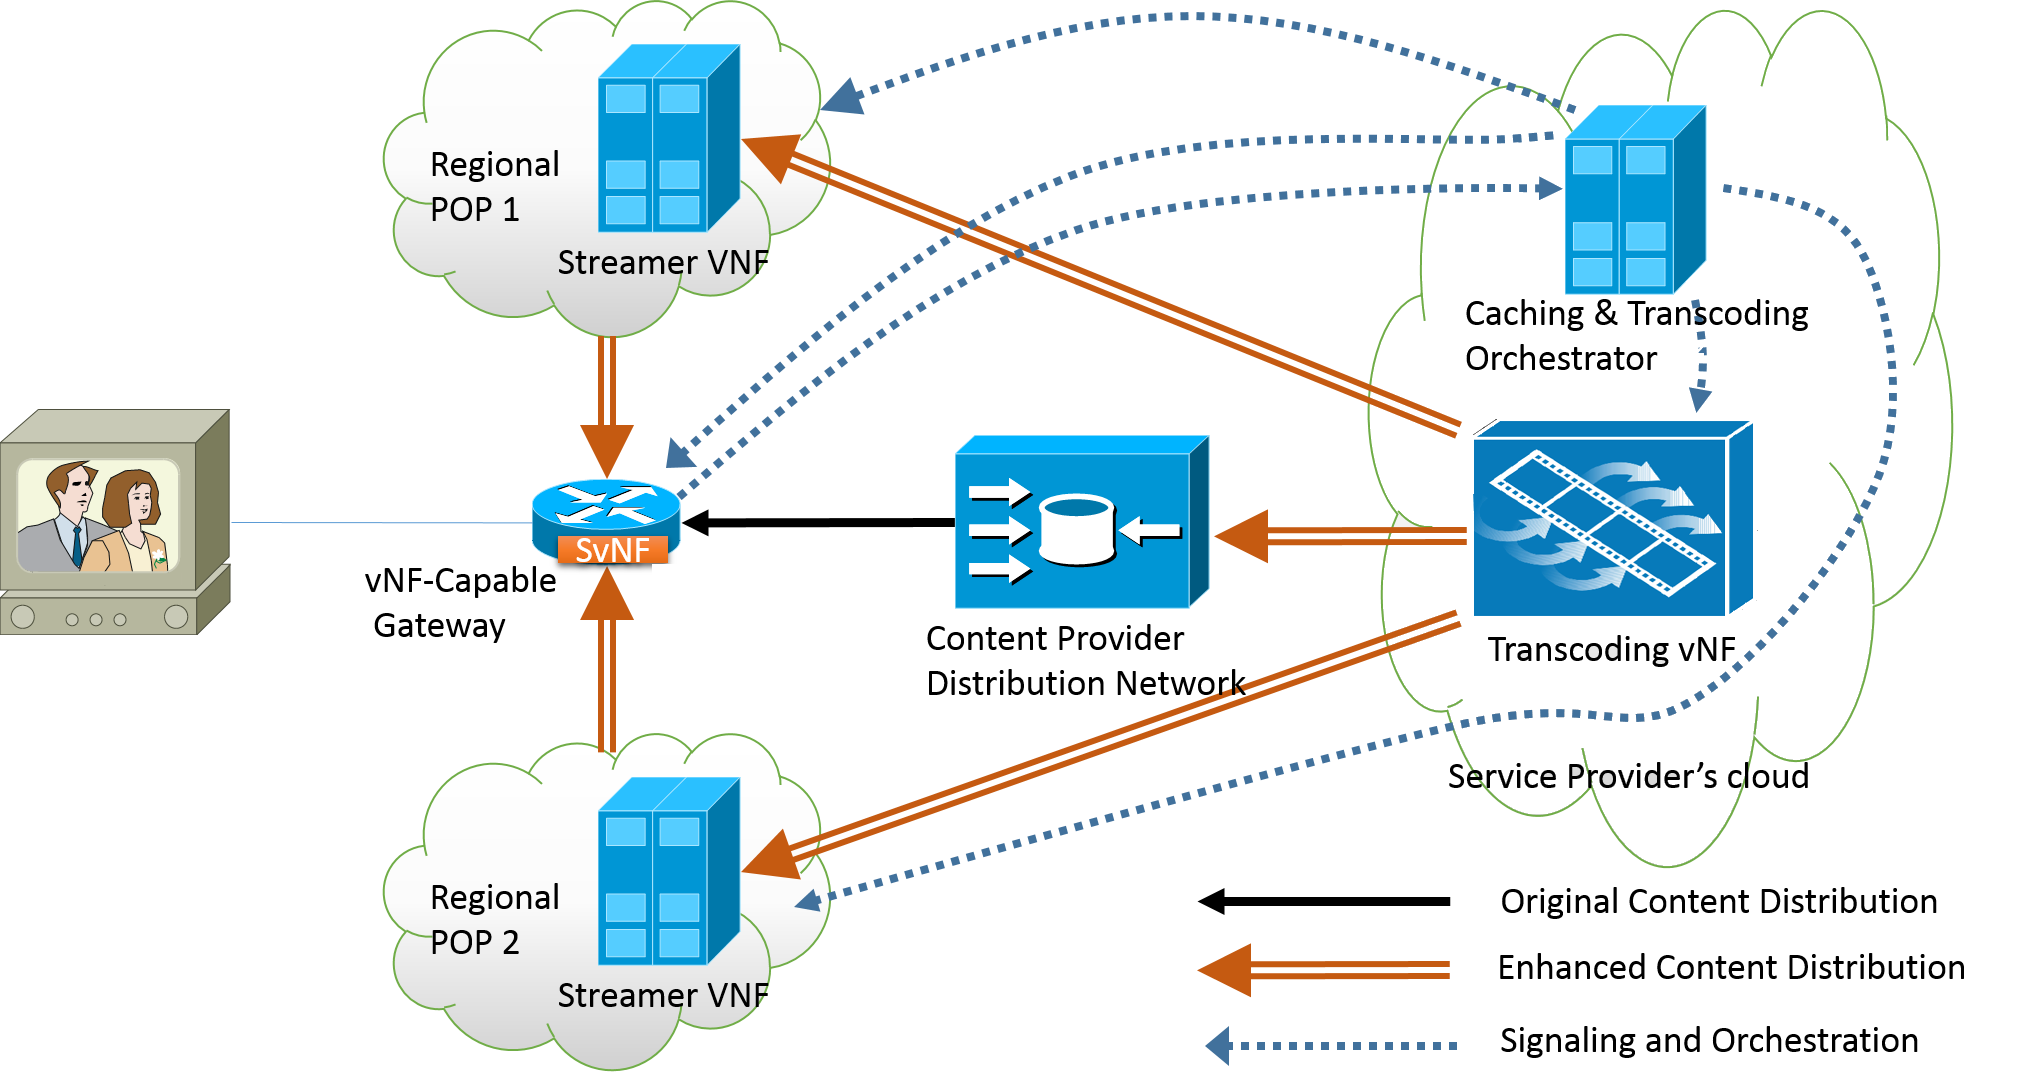
\includegraphics[width=0.95\linewidth]{highleveldesign7.png}
	\vspace{2em}
	\setbeamercolor{block title}{bg=applegreendark}
	\begin{block}{}
		Finally, all the building blocks collaborate to deliver the best version of the media from the best location in the network.
	\end{block}
\end{frame}


\begin{frame}{Feasibility study}
	\begin{columns}[T]
		\begin{column}[T]{0.55 \textwidth} 
			\vspace{1em}
			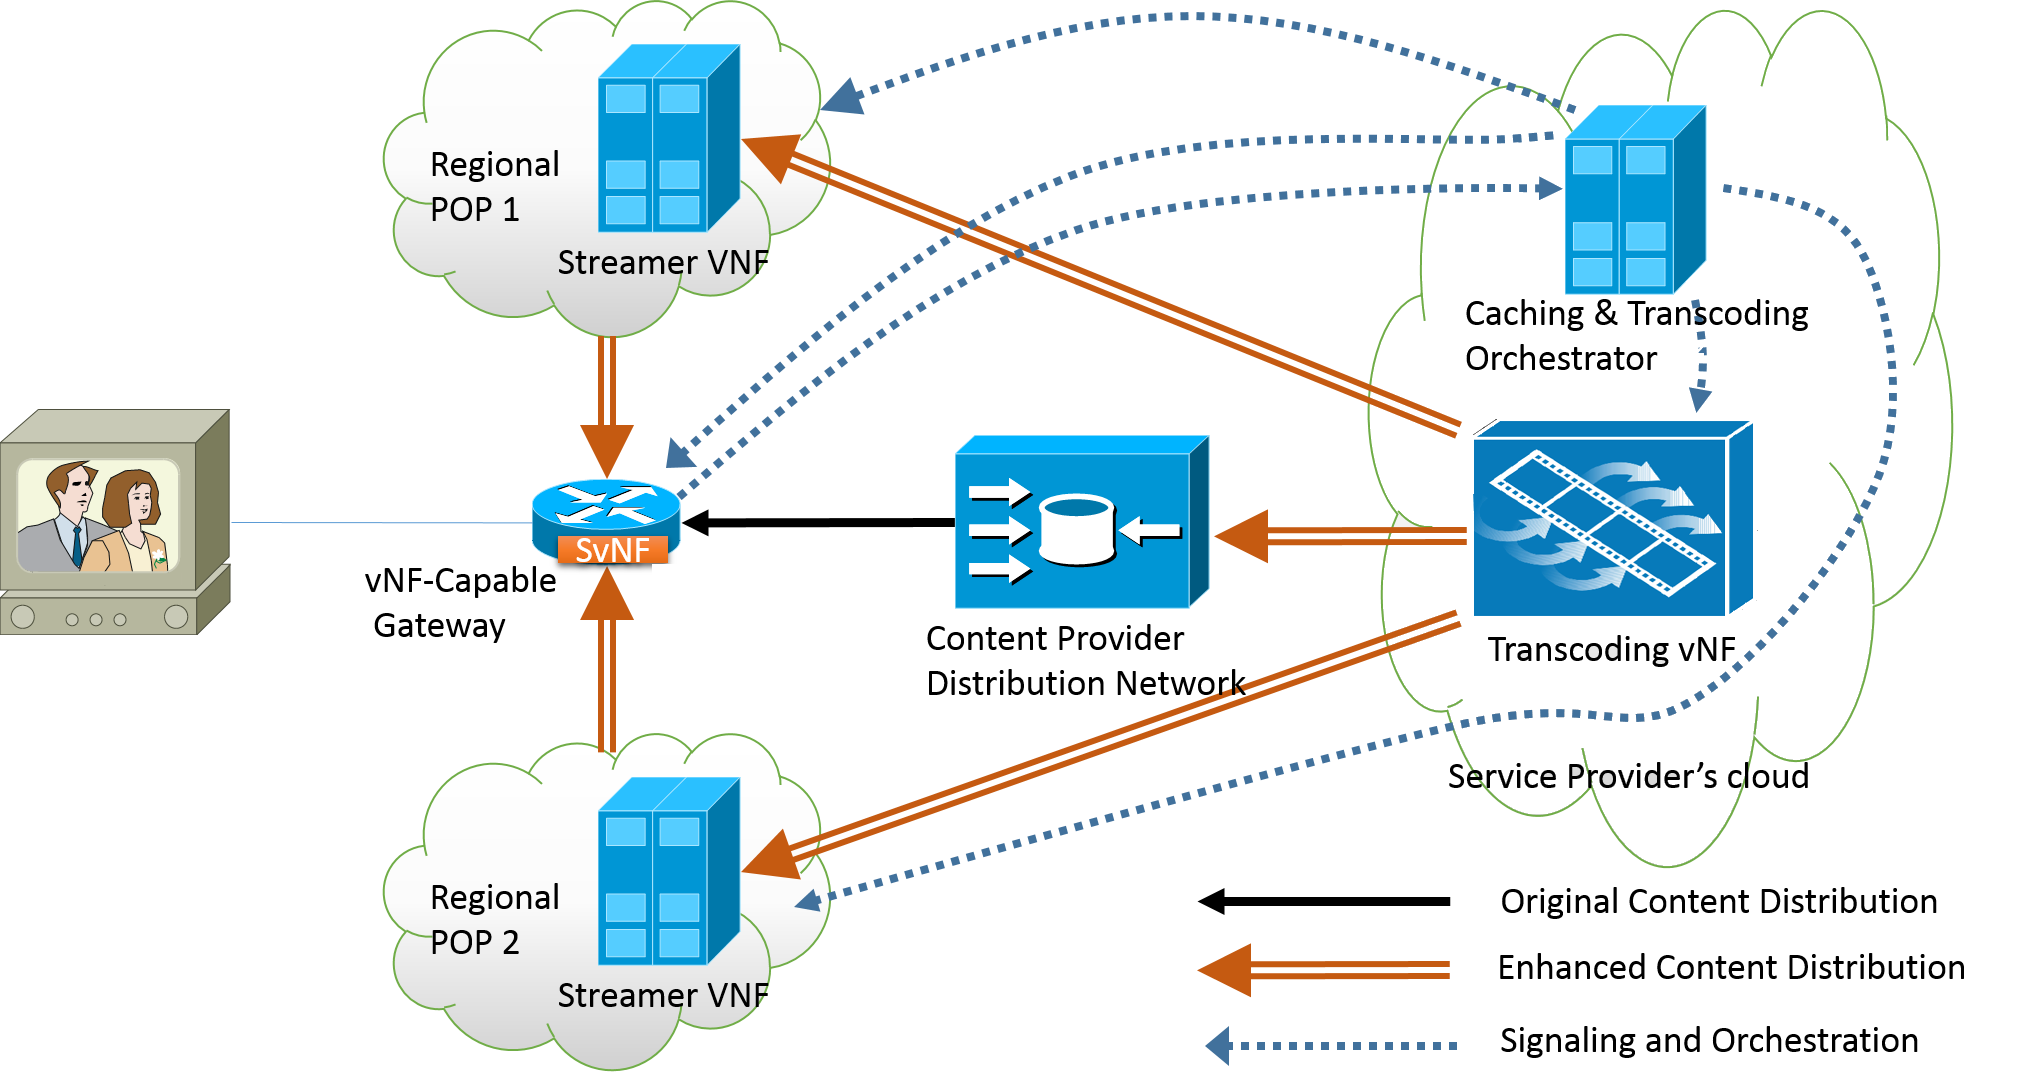
\includegraphics[width=18em]{highleveldesign7.png}
		\end{column}
										
		\begin{column}[T]{0.35\textwidth} 
										   
			\textbf{Topics we address in the evaluation}
			\begin{itemize}
				\item How does the SvNF fits on the HG?
				\item What is the value brought by the overall service?
				\item How do we optimize service operations?
			\end{itemize}
		\end{column}
																										
	\end{columns}
								
\end{frame}

\begin{frame}{We generated traffic to a gateway with SvNF deployed and compared key metrics}
\begin{columns}[t]
				\begin{column}[T]{0.90 \textwidth}
				\centering
				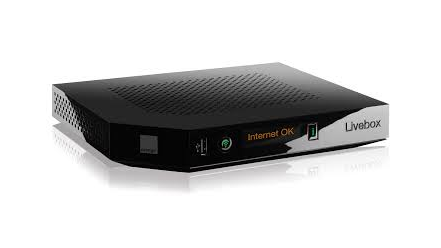
\includegraphics[height=5em]{livebox.png}					
				\end{column}
				
			\end{columns}

	\resizebox{\linewidth}{!}{
	\begin{tabular}{ c |c |c |c || c |c |c |}
	
	
 	     & \multicolumn{3}{c}{Web Traffic} 		  & \multicolumn{3}{c}{File Transfer} \\
 	     \cline{2-7}	
              & CPU  			& free Memory 	& Throughput & CPU 		& Free Memory & Throughput  \\
              & baseline = 1 			& baseline = 693 MB		& baseline=11.5 MBps	&  		&  baseline = 708 MB		& baseline =  11.5 MBps \\\hline   
Baseline   &   1x 		  & 100\% 		& 100 	    & 1x		& 100\% 		& 100 \\\hline
Squid &   14x        & 99\% 		& $\simeq$100		& 17x		& 99.3\% 		& $\simeq$100 \\\hline
\textbf{SvNF} &   \textbf{18x}		  & 98\% 		& 99.5		& \textbf{20x}		& 99.8\%		& $\simeq$100 \\\hline
\textbf{SvNF with rules}&   \textbf{19x}        & 99\% 		& 99.7		& \textbf{21x}		& 99.4\%		& $\simeq$100 \\\hline
	
	            
	\end{tabular}
	}
	
\vspace{0.5em}
\small{		SvNF HTTP Proxy vs Squid HTTP Proxy vs Baseline Performances Comparison}
\vspace{2.5em}
	\begin{block}{}
		The study shows stable performance and low memory footprint but a high CPU utilization. Modern HG can support the load without error or added latency.
	\end{block}
	
								
\end{frame}

\begin{frame}{We simulated 2 scenarios to evaluate overall performances by counting SLA violations}
	
			

		\begin{columns}[T]
		\begin{column}[T]{0.33 \textwidth} 
			
			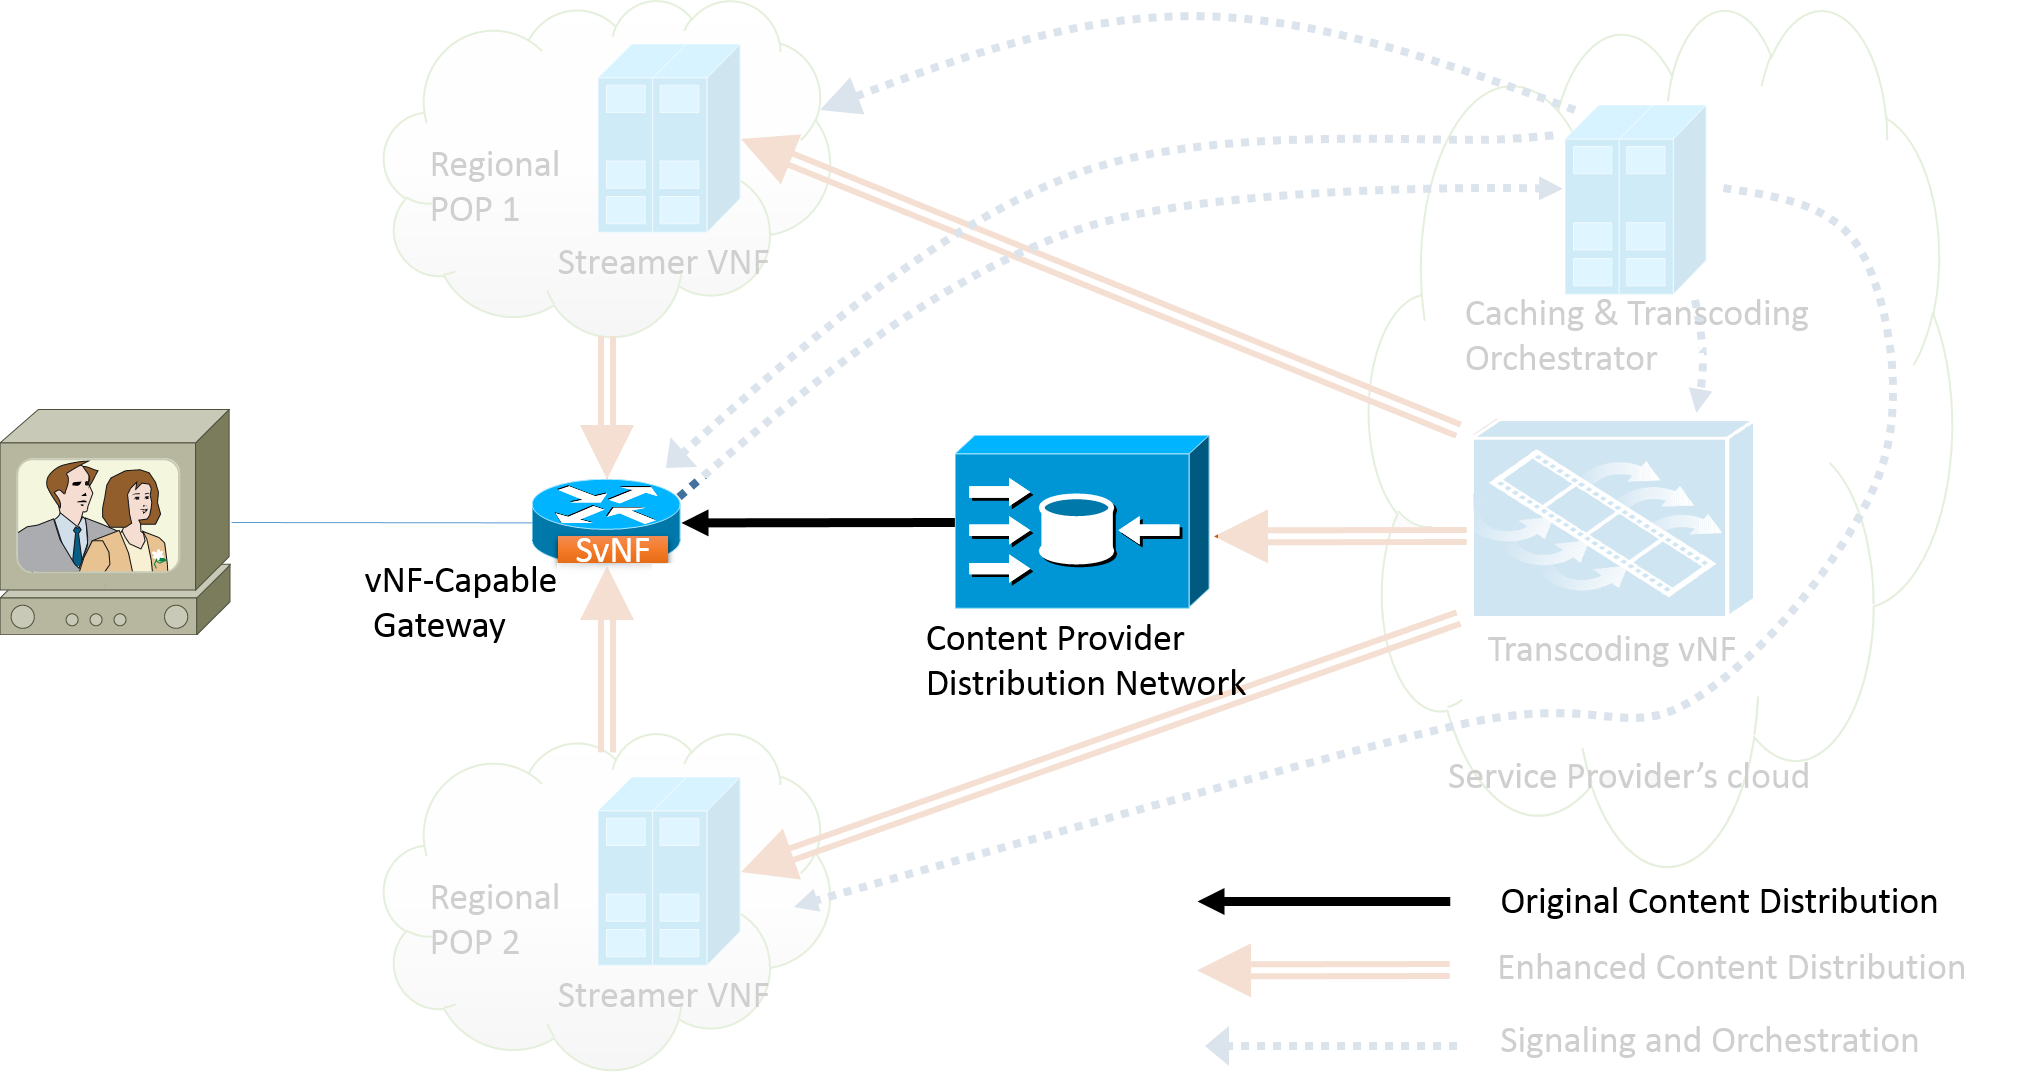
\includegraphics[width=10em]{highleveldesign1.png}
		\end{column}
										
		\begin{column}[T]{0.66\textwidth} 
										  
			\textbf{Scenario A}
			\begin{itemize}
				\item All the media are consumed through a link with CP Network
				\item 50ms latency / 2Gbps bandwidth
			\end{itemize}
			\vspace{3mm}
			
		\end{column}
																										
	\end{columns}
	
		\begin{columns}[T]
		\begin{column}[T]{0.33 \textwidth} 
		\vspace{2em}
			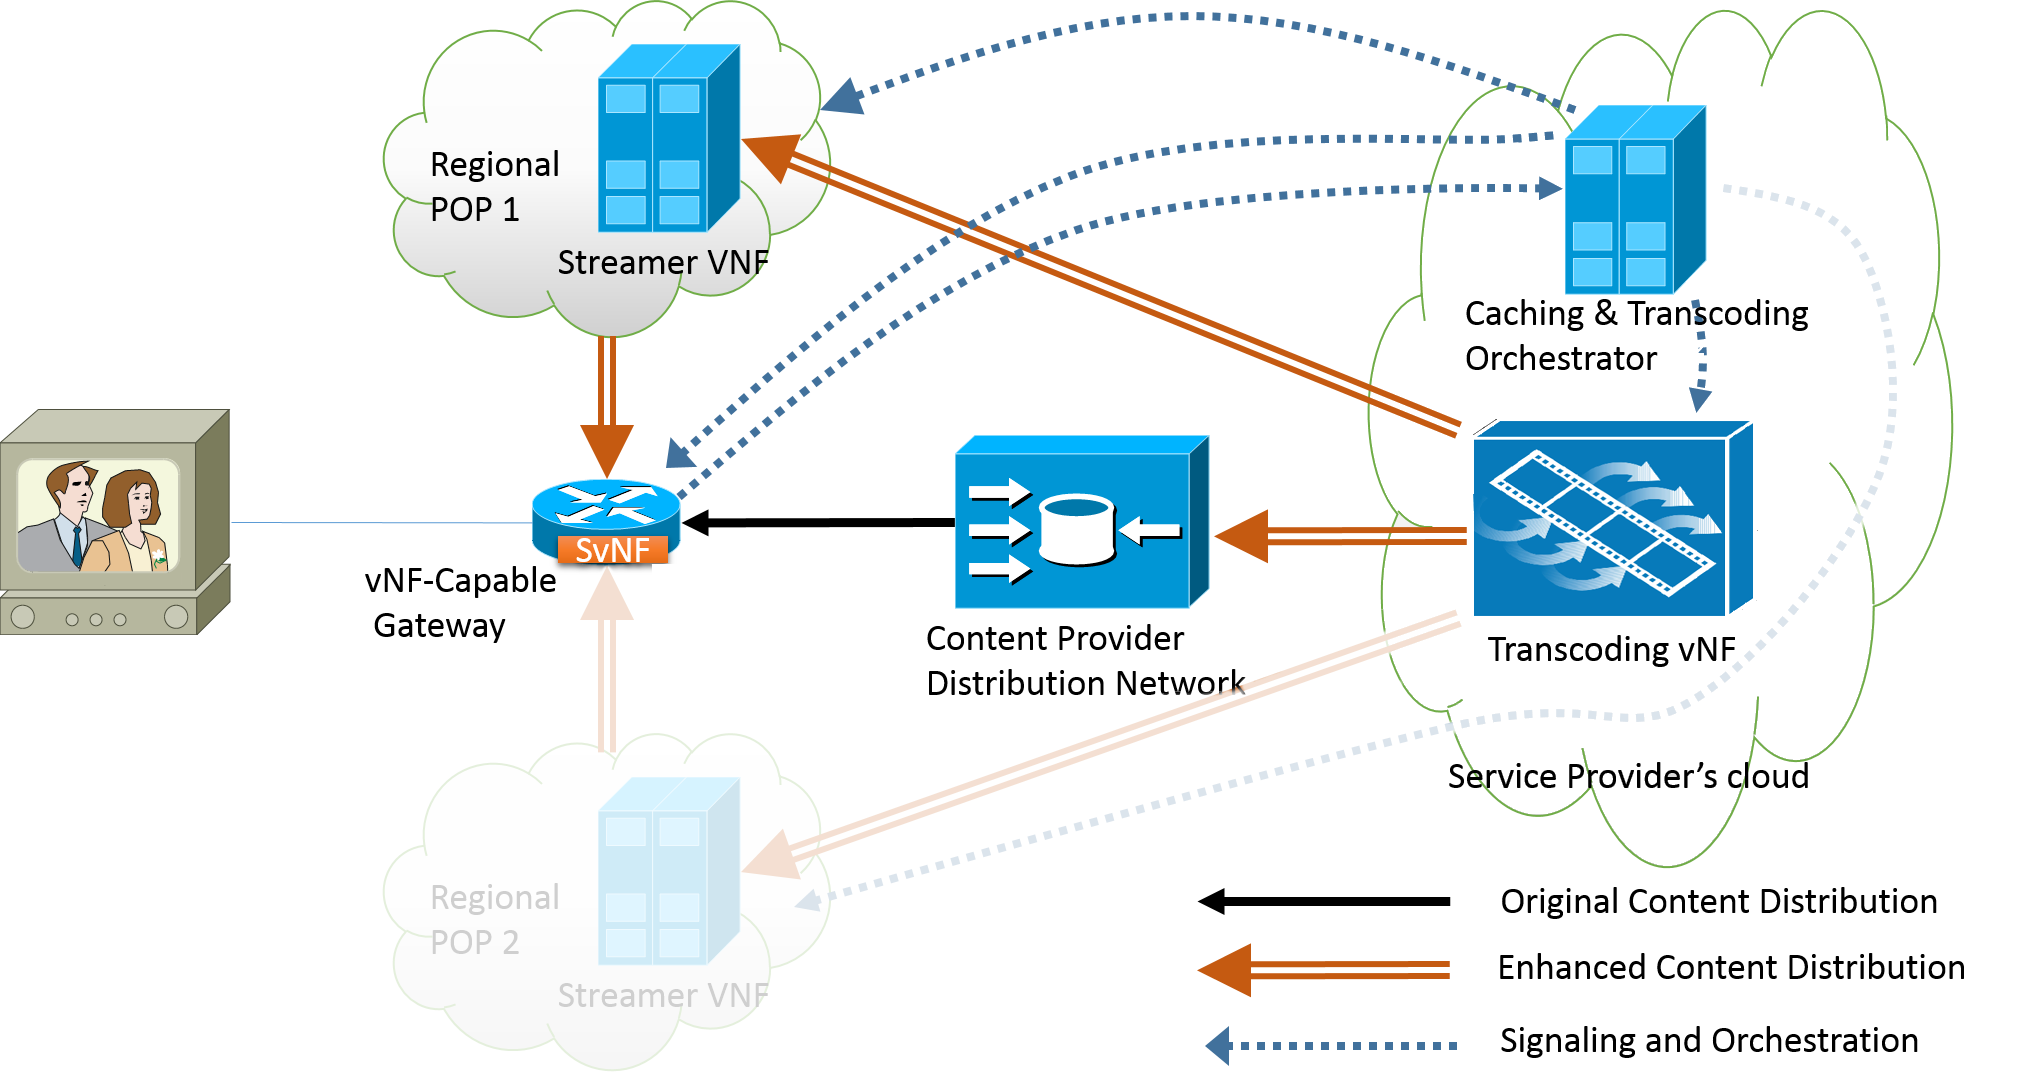
\includegraphics[width=10em]{highleveldesign7bis.png}
		\end{column}
										
		\begin{column}[T]{0.66\textwidth} 
										  
			\textbf{Scenario B}
			\begin{itemize}
				\item Media is consumed from the CP Network and from vNF Streamer on PoP
				\item For CP: 50ms latency / 1Gbps bandwidth
				\item For PoP: 25ms latency / 1Gbps bandwidth
				\item Media is cached in PoP after 4 cache miss
			\end{itemize}
			
		\end{column}
																										
	\end{columns}
	
	
	
\end{frame}

\begin{frame}{Assumptions}
	
			

  
		\begin{itemize}
			\item Content Provider allow provisionning content in Service Providers Network
			\item Simulation has been implemented with NS3
			\item 200 Gateways
			\item 300 Videos
			\item SLA Violation criteria: less than 75\% of the target bitrate 10s after the request
		\end{itemize}
										  
			
	
	
	
\end{frame}

\begin{frame}{For the same bandwidth, our proposal - Scenario B - shows a drastic diminution of SLA violations.}
	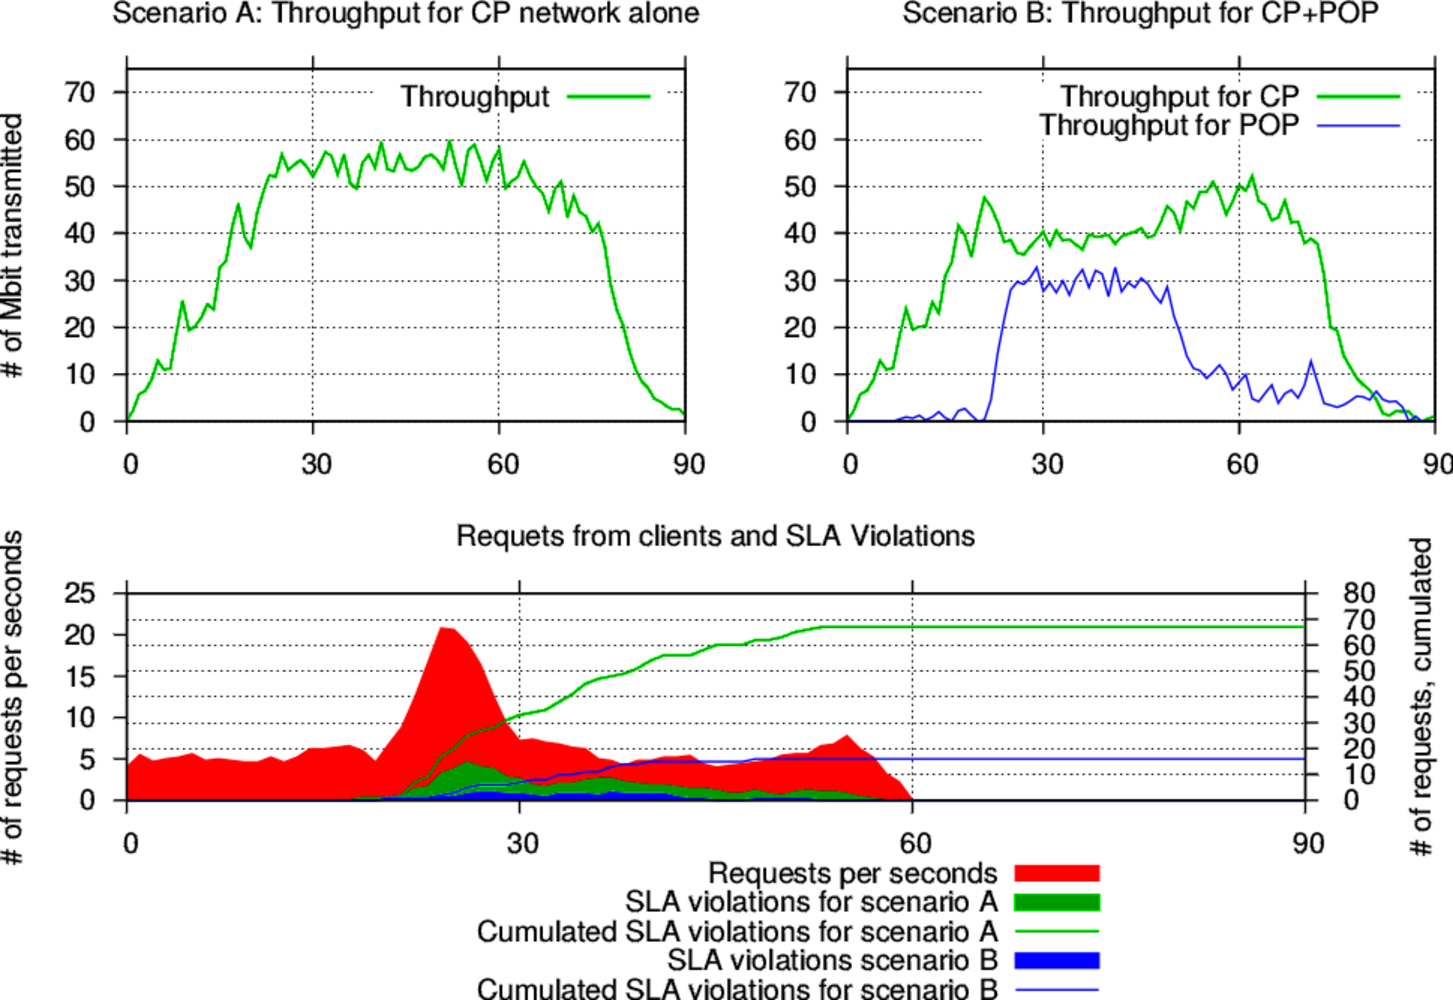
\includegraphics[width=0.90\linewidth]{CP+POP_evaluation.pdf}
\end{frame}

\begin{frame}{For the same bandwidth, our proposal - Scenario B - shows a drastic diminution of SLA violations.}
	\includegraphics[width=0.90\linewidth]{CP+POP_evaluation.pdf}
		\begin{textblock*}{8cm}(3cm,0.4\textheight)
		\begin{alertblock}{}
			\textbf{ Is that really a surprise? }
			\begin{itemize}
				\item No: we considered streaming over HTTP, so delay is key and favor the PoP over CP.
				\item But, being located in SP network limit hops and delay, and cross-ISP trafic
				\item \textbf{So deploying this solution with the NFV approach offers both low cost and flexibility to SP.}
			\end{itemize}
		\end{alertblock}
	\end{textblock*}		
\end{frame}

\begin{frame}{Provisioning decision highly impact the performance of the solution}
	\includegraphics[width=0.90\linewidth]{cachingStrat_evaluation.pdf}
		\begin{columns}[T]
		\begin{column}[T]{0.5 \textwidth} 
		
		\textbf{Provisioning too early}
			\begin{itemize}
				\item Each time a video is asked
				\item Streamer vNF is saturated with requests that could have been served by CP
			\end{itemize}
		\end{column}
										
		\begin{column}[T]{0.5\textwidth} 
										  
			\textbf{Provisioning too late}
			\begin{itemize}
				\item Cached only when a big number of user ask for a video
				\item Stream vNF is underused, CP network can't handle the load
			\end{itemize}
			
		\end{column}
																										
	\end{columns}
\end{frame}

\begin{frame}{Provisioning decision highly impact the performance of the solution}
	\includegraphics[width=0.90\linewidth]{cachingStrat_evaluation.pdf}
		\begin{columns}[T]
		\begin{column}[T]{0.5 \textwidth} 
		
		\textbf{Provisioning too early}
			\begin{itemize}
				\item Each time a video is asked
				\item Streamer vNF is saturated with requests that could have been served by CP
			\end{itemize}
		\end{column}
										
		\begin{column}[T]{0.5\textwidth} 
										  
			\textbf{Provisioning too late}
			\begin{itemize}
				\item Cached only when a big number of user ask for a video
				\item Stream vNF is underused, CP network can't handle the load
			\end{itemize}
			
		\end{column}
																										
	\end{columns}
	
		\begin{textblock*}{8cm}(3cm,0.4\textheight)
		\begin{alertblock}{}
			\textbf{ Can other parameters be considered? }
			\begin{itemize}
				\item Yes: other video meta-data can be useful
				\item Solution could be augmented with a push-based provisioning where popular video could be provisioned before publication
				\item But local video popularity account for most of the predictability for growing demand
			\end{itemize}
		\end{alertblock}
	\end{textblock*}		
	
\end{frame}

\begin{frame}{Conclusion and future work}
	\begin{columns}[T]
		\begin{column}[T]{0.33 \textwidth} 
			\vspace{5em}
			\includegraphics[width=10em]{conclusion.jpg}
		\end{column}
										
		\begin{column}[T]{0.66\textwidth} 
										   
			\textbf{Advantages of SvNF+NFV approach}
			\begin{itemize}
				\item Standard-based (HGI, OSGI, ETSI NFV)
				\item Pragmatic migration path to fully virtualized Home Gateway
				\item Real use case bringing new service to SP
			\end{itemize}
			\vspace{3mm}
			\textbf{Future Work}
			\begin{itemize}
				\item Investigate more basic Network Functions
				\item Collaboration between SP and Content Delivery Network
				\item Other execution environments
			\end{itemize}
																																						
		\end{column}
																										
	\end{columns}
	

	
\end{frame}

\begin{frame}{Conclusion and future work}
	\begin{columns}[T]
		\begin{column}[T]{0.33 \textwidth} 
			\vspace{5em}
			\includegraphics[width=10em]{conclusion.jpg}
		\end{column}
										
		\begin{column}[T]{0.66\textwidth} 
										   
			\textbf{Advantages of SvNF+NFV approach}
			\begin{itemize}
				\item Standard-based (HGI, OSGI, ETSI NFV)
				\item Pragmatic migration path to fully virtualized Home Gateway
				\item Real use case bringing new service to SP
			\end{itemize}
			\vspace{3mm}
			\textbf{Future Work}
			\begin{itemize}
				\item Investigate more basic Network Functions
				\item Collaboration between SP and Content Delivery Network
				\item Other execution environments
			\end{itemize}
																																						
		\end{column}
																										
	\end{columns}
	
	
	\pause
	
			\begin{textblock*}{11cm}(1cm,20em)
		\begin{block}
		
			\textbf{ ~~~~~~~~~~~~~~~~~~~~~~~~~~Questions? \\Nicolas Herbaut, LaBRI Bordeaux France, nherbaut@labri.fr}
			
		\end{block}
	\end{textblock*}	
	
\end{frame}

\begin{frame}{Backup Slides}
	
\end{frame}

\begin{frame}{Simulation Hypotheses}
	\resizebox{\linewidth}{!}{
	
	
		\begin{tabular}{| l | l | l|}
		\hline
			\textbf{Settings} & \textbf{Scenario A} & \textbf{Scenario B}\\\hline
			CP Bandwidth &2 Gbps&1 Gbps\\\hline
			Regional PoP Bandwidth &0 Gbps&1 Gbps\\\hline
			Regional PoP latency& \multicolumn{2}{l|}{25ms} \\\hline
			CP latency& \multicolumn{2}{l|}{50ms} \\\hline
			Video Distribution& \multicolumn{2}{l|}{Normal} \\\hline
			Video Size&\multicolumn{2}{l|}{Pareto with average video size=10Mb}\\\hline
			Requested bitrate &\multicolumn{2}{l|}{320kbps}\\\hline
			\# of gateways &\multicolumn{2}{l|}{ 200}\\\hline
			\# of video (cruising/peak) &\multicolumn{2}{l|}{ 200/100}\\\hline
			Mean time between request (cruising/peak) &\multicolumn{2}{l|}{ 0.1s/0.05s (Poisson))}\\\hline
			SLA Violation criteria &\multicolumn{2}{l|}{ less than 75\% of the target bitrate 10s after the request}\\\hline
			Video Caching&\multicolumn{2}{l|}{after 4 requests}\\\hline
		\end{tabular}
	
	

	}
	
\end{frame}


\end{document}


